\chapter{Implementation and Evaluation of Capacity Sizing}
\label{chap:impl}

This chapter considers two example sensing applications and the design of wireless sensor systems to achieve the goals of these applications.
We explore the system design for these applications within the context of the conclusions of \cref{chap:intuition,chap:capacity,chap:battery}, which suggest that energy capacity is highly important for energy harvesting wireless sensor performance.
The first application that we consider is the measurement of fine-grained workplane illuminance. These illuminance measurements are used to inform the operation of a lighting control system to balance artificial and natural light for occupant's workplanes. 
The goals of this application are to measure illuminance at high granularity with high availability and provide a lifetime of at least a decade. 
This application is relatively simple and it is used to validate the simulation and conclusions presented in \cref{chap:intuition,chap:capacity}.
The second application is image-based human occupancy detection and counting. 
Human occupancy measurement can help inform building energy management and climate control.
The goal of this application is to accurately and consistently detect the presence of humans within view while providing a lifetime of several years.
This application considers an existing batteryless image sensing solution and reconsiders their design in the context of the conclusions of previous chapters.
We propose designs for each of these applications, and detail their implementation and evaluation.
Utilizing a hybrid energy harvesting architecture with sufficient rechargeable energy buffer and a backup non-rechargeable energy storage, our proposed sensor designs are able to provide significantly higher availability than batteryless designs, as well as much longer lifetimes than battery-based designs. 

\section{Measuring Workplane Illuminance}
\label{sec:impl:permamote}

%We discuss the implementation of both the model used to generate the results
%of \cref{sec:store} and \cref{sec:primary}, and the \name hardware that
%is based on these results. All of our hardware and software will be made
%\textbf{open source} for use by other researchers.


\begin{definefigure}{fig:permamote}
    \centering
    \begin{subfigure}{0.7\columnwidth}
        \centering
        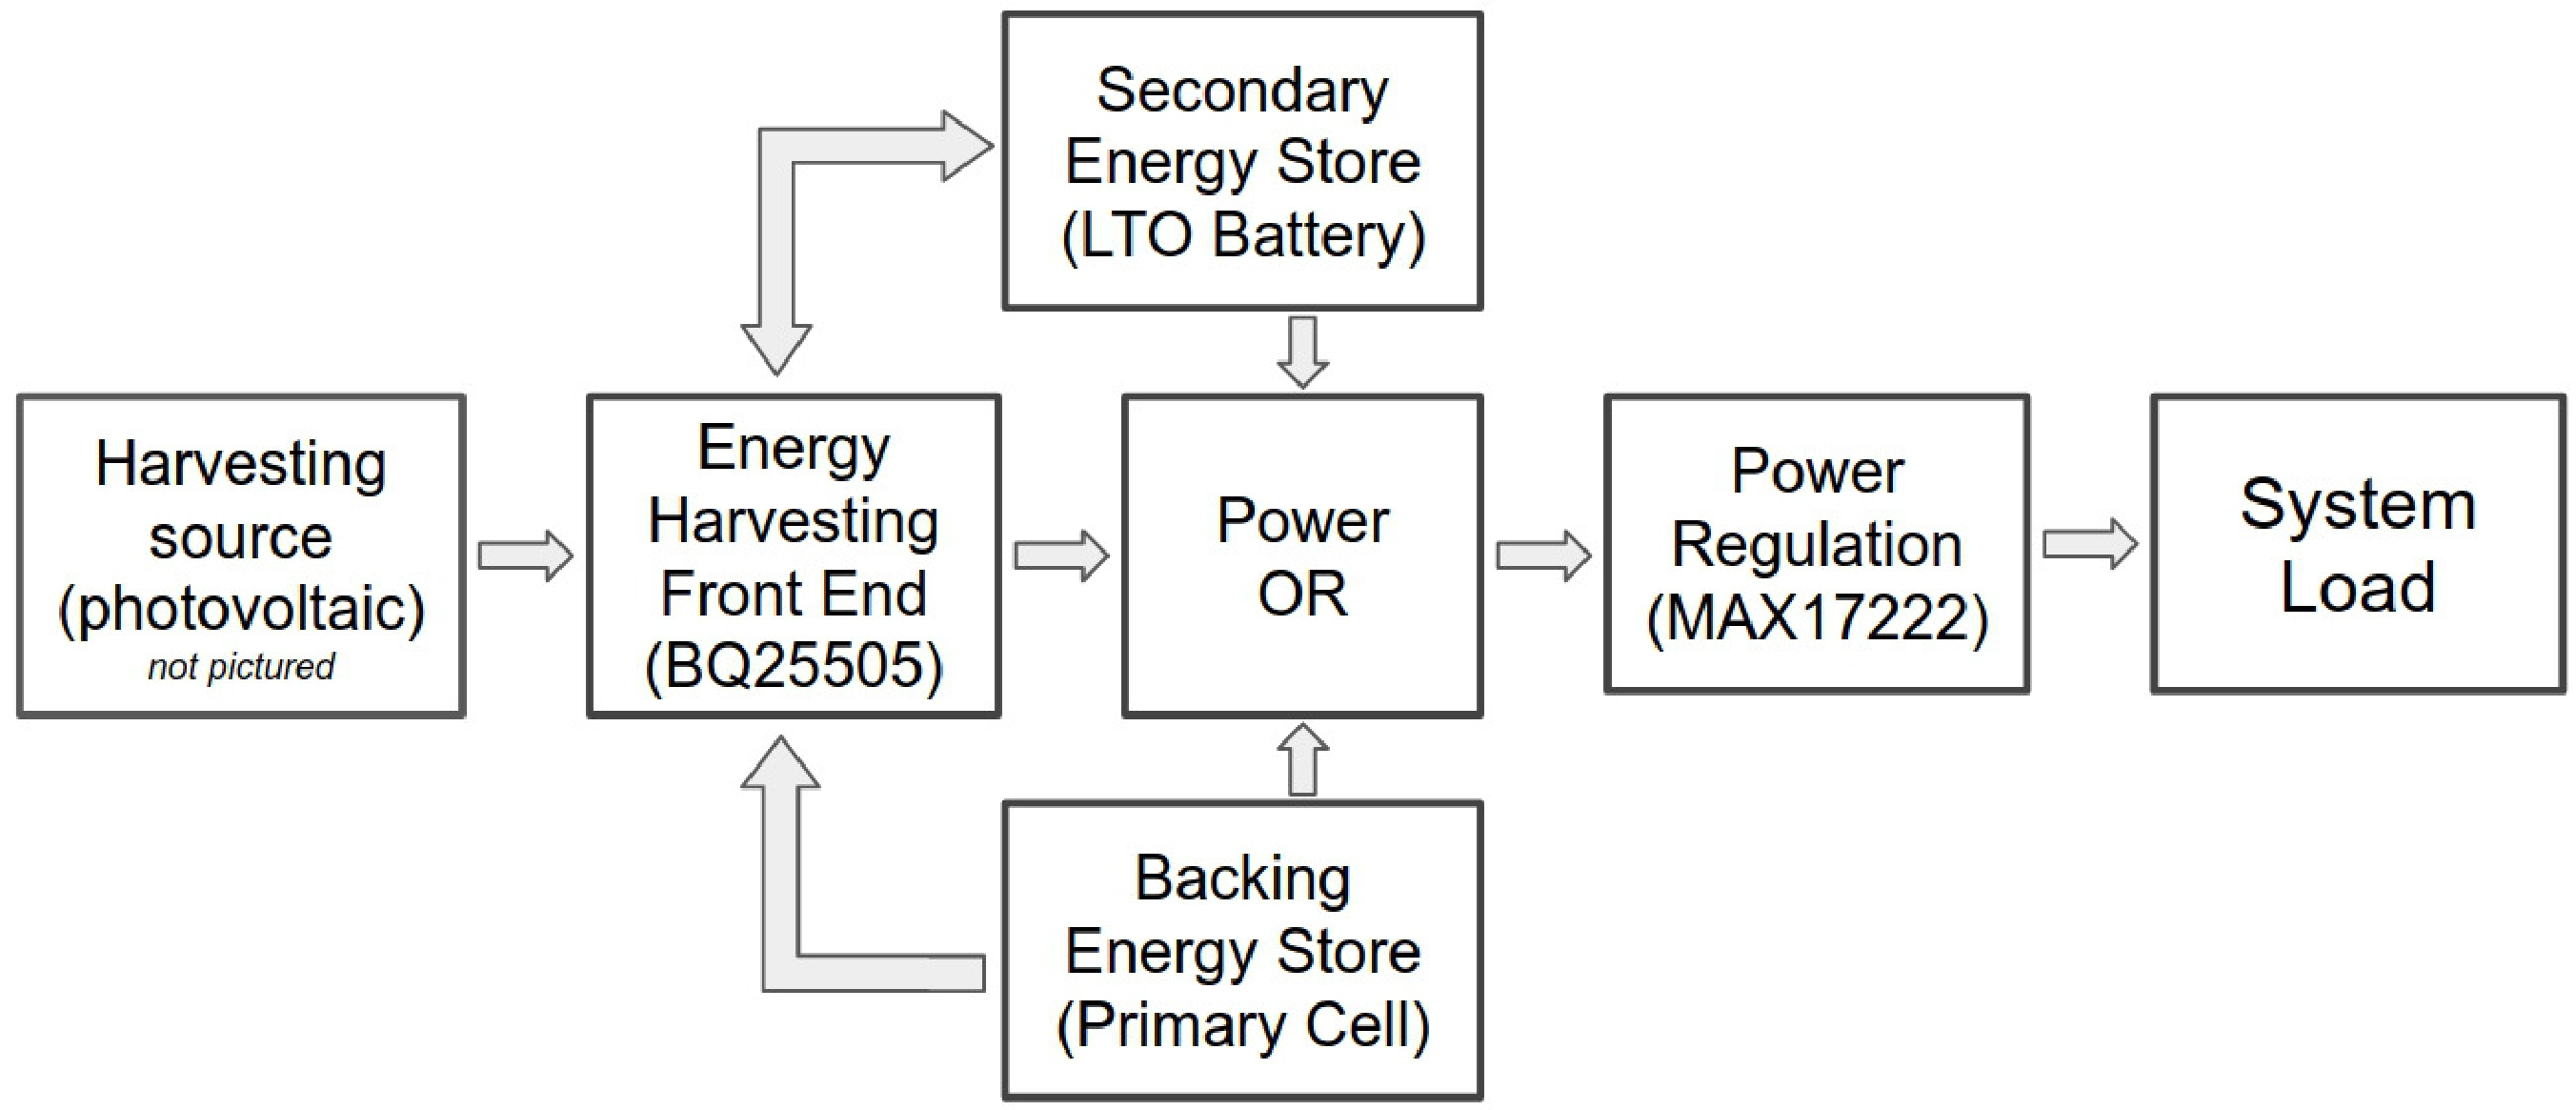
\includegraphics[width=\textwidth]{figs/capacity/arch}
        \caption{Harvesting and storage architecture}
    \end{subfigure}
    \begin{subfigure}{0.29\columnwidth}
        \centering
        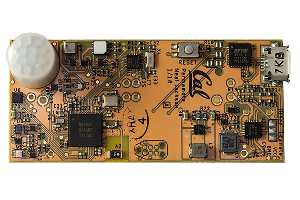
\includegraphics[width=\textwidth,angle=90]{figs/capacity/permamote}
        \caption{Hardware}
    \end{subfigure}
    \caption{\normalfont The \name power supply architecture is informed by the
    findings in \cref{chap:intuition,chap:capacity,chap:battery}. An
    LTO battery is recharged by a solar panel. When the battery is depleted,
    a primary-cell powers the system, providing reliability and avoiding
    intermittency.
    }
    %We believe this platform will run for 6-36 years for common
    %sensing tasks and indoor lighting conditions before the death of
    %the primary-cell. Even after the primary-cell expires,
    %the sensor node could continue to run batterylessly on harvested energy.
\end{definefigure}

The advent of LED lighting has significantly reduced electricity consumption in residential and commercial sectors. However, residential and commercial lighting still consumes 5\% of the \textit{total} U.S. electrical consumption~\cite{aeo2022}.
Beyond the utilization of LED lighting, the technique of daylighting, or lighting buildings with natural light, can further reduce the amount of electricity consumed by buildings. 
Since the intensity of daylight can be unpredictable as it depends on weather, it can be difficult to achieve consistent lighting with natural light alone.
Artificial lighting can be used to augment insufficient natural light, but it requires fine-grained measurement to provide feedback to control and maintain a set point in a space.
In particular, workplane illuminance for commercial buildings is important for occupant comfort and productivity, but is difficult to maintain with existing lighting control systems. 
Modern lighting control systems that perform both measurement and control are generally limited to large zones of measurement and influence. 
The cost of instrumentation and automation is often too exorbitant to justify fine-grained more fine-grained focus.
This often results in inequitable and sometimes uncomfortable lighting for occupants.
Wireless sensing could provide a solution for fine-grained workplane measurement for daylighting applications, assuming the sensor does not require frequent maintenance and provides high availability and consistent measurements for the lighting system feedback loop.
For this specific example, our application goals are to provide at least a ten year lifetime with consistently high availability. 
This section details the realization of a design to meet these requirements, and utilizes this design to verify our the results of the simulation and design conclusions detailed in earlier chapters.

\placefigure{fig:permamote}

\subsection{Design and Implementation}
We design and implement a prototype sensor named \name to perform workplane illuminance sensing based on the application requirements described previously and the design principals discussed in \cref{chap:capacity,chap:battery}.
%The \name sensing platform
%utilizes the components from the representative hardware listed in \cref{tab:capacity:components} 
%used in our simulation. 
\name integrates a processor, BLE/802.15.4 radio, and various environmental, lighting,
and a passive infrared (PIR) occupancy sensor.
The components used in \name are the same ones that we used to develop our representative hardware and workloads for our simulation. 
These components are listed in \cref{tab:capacity:components}. 
A picture
and system diagram of \name is shown in \cref{fig:permamote}. All hardware
and software for the platform is open source\footnote{\url{https://github.com/lab11/permamote/tree/master/hardware/permamote}}.

\placefigure{fig:impl:permamote_life}
\subsubsection{Energy Harvesting and Storage.}
Some of the primary goals of \name are to provide workplane illuminance measurements with high availability for a long lifetime of greater than ten years. 
Given the results of our simulation, a design that relies solely on energy preallocation is unlikely to achieve a sufficiently long lifetime. 
\name is powered by an energy harvesting front end that capitalizes on the benefits
of rechargeable and non-rechargeable energy capacity. 
It utilizes the TI BQ25505 energy harvesting IC, which
harvests energy while monitoring both
rechargeable and backup energy stores,
switching between them at user-configurable voltage thresholds~\cite{bq25505}. 

We utilize the hueristics developed in \cref{sec:intuition:capacity} to determine the required sizing for our energy harvesting and energy storage. 
We select a 10.9\ssi{\centi\meter\squared} amorphous
silicon photovoltaic panel as our energy harvester to fit within our form factor.
Assuming the lower end of efficiency (10\%) and the upper bound of indoor irradiance, this panel can provide an average of 100\ssi{\micro\watt}. 
On average, this income power provides more than sufficient average power to support various frequencies of the sense and send workload.
We can consult \cref{sec:intuition:capacity,sec:capacity:capture} to estimate the minimum required capacity for the sense and send workload.
Considering the average power required by the sense and send workload with a 30 second period (24.5\ssi{\micro\watt}), 
the minimum sufficient capacity should be \num{1.4E3} times the average workload power. 
This is if we assume an income distribution similar to the EnHANTs Setup D and an income margin of 300\% of the expected workload power\footnote{100\ssi{\micro\watt} represents a 300\% margin over the 24.5\ssi{\micro\watt} workload}.
This suggests the capacity of the rechargeable energy storage should be on the order of 34\ssi{\milli\Wh}.
This agrees with results from our simulation in \cref{fig:capacity:availability} suggesting energy capacity on the order of 1--10\ssi{\milli\Wh} will be sufficient to achieve near perfect availability in conditions like Setup D captures.
The simulation suggests slightly less capacity is required compared to the heuristic estimate.
This is because the simulations assume the energy buffer starts fully charged.
Most systems, especially those that rely on rechargeable batteries, are deployed fully or partially charged.
In our simulation, this provides an influx of energy into the system and it does not need to capture as much harvested energy to power its workload, and thus requires less energy capacity.
If simulated for more time, over a longer period than the energy income trace provides, the capacity determined by simulation results may not be sufficient to continue an energy neutral operation.
The heuristic for energy capacity sizing provides a safer, more conservative estimate. 

Given this analysis, we select a 20\ssi{\milli\Ah} (48\ssi{\milli\Wh}) LTO battery 
to achieve this energy capacity~\cite{LTODatasheet, LTODatasheet2}.
As described in \cref{sec:battery:life},
we configure the voltage thresholds of the BQ25505 to derate the 
usable capacity of this battery to  
increase the apparent cycle lifetime of the battery. 
The resulting energy storage provides 24\ssi{\milli\Wh} of
energy storage, more than the capacity required to achieve the reliability and energy utilization
improvements of the workloads that were simulated in \cref{sec:capacity:primary,fig:capacity:primary}.

In some cases, the available harvestable power may be lower than expected and insufficient to operate in an energy neutral fashion. 
This justifies the addition of a reliable, non-rechargeable backup energy source.
\Cref{fig:impl:permamote_life} is a recreation of \cref{fig:capacity:primary} presenting the estimated lifetime of \name with its configured 24\ssi{\micro\Wh} rechargeable storage and various non-rechargeable backup energy storage options. We assume a 30 second sense and send workload period.
From this simulation result, \name requires at least one CR2032 coin cell to achieve the application lifetime goals in the worst case energy harvesting potential.
Thus, \name is designed to be configured with either one or two CR2032 coin
cells or a CR123A cell. 
%Primary-cells provide 3-13x more density and 2-12x less
%leakage than a secondary-cell.
%making them more desirable than a single,
%large, pre-charged secondary-cell as the backup store~\cite{LTODatasheet,primary2032, primarycr123a}.
The output of the active battery
is boosted by a MAX17222 regulator, which features high conversion efficiency
(>90\%) at low output currents and operates down to 400\,mV~\cite{max17222}.
%We have the ability to monitor harvesting and system currents using
%the iCount method by sensing the voltage of
%the inductor used by the BQ25505 and MAX17222~\cite{duttaEnergy08}. The processor
%is also capable of gating all sensors from the main power supply to save
%power.\\

\subsubsection{Processor, Radio and Sensor Selection}
In designing \name, we strive to select modern and low power components.
%We feel that it may
To benefit other
platform builders, we document our component selections
along with their key performance metrics. A summary of these
components can be found in \cref{tab:capacity:components}.

We note our choice of the Nordic NRF52840 MCU over the more commonly used MSP430FR series
because of its higher active power efficiency while offering comparable sleep currents.
Specifically, it only draws 56\,\uA/MHz compared to over 100\,uA/MHz
for the MSP430, which is a common choice for batteryless systems. 
Unlike batteryless systems,
\name is designed with sufficient rechargeable capacity and backup energy and is intended to never power off and lose volatile state. 
This eliminates any reliance on state retention techniques and the need for the non-volatile FRAM present on the MSP430FR series chips. 
While
slightly more efficient
processors and radios exist than those found in the NRF52840,
we value the simplicity of the SoC-based design as well the platform's capability of using either BLE or 802.15.4 over its 2.4\ssi{\giga\hertz} radio.  

\subsection{Simulation Evaluation using Real Systems}
\label{sec:eval}
To evaluate our simulation and the benefits of a capacity-focused design, 
we perform a three-month-long deployment in a partially sunlit room
using i) a primary-cell only system~\cite{adkins2015michigan}, ii) a batteryless, capacitor-only system~\cite{campbellEnergy14}, and iii) \name, our
system that features both a secondary and primary-cell. 
We model these
systems over the same period using estimated irradiance from \name illuminance masurements. 
We compare the performance and lifetime of these three systems with the predictions generated by a simulation of their workload. 
We also compare the availability of \name to the batteryless system.

%\subsubsection{Simulating Sense and Send with \name}
%We perform benchmarks on the \name platform to develop the workloads presented in \cref{sec:capacity:modelling}.
%The workplane illuminance measurement application represents the same periodic sense and send workload used in our simulation.
%\name requires a total of 586\ssi{\micro\joule} to measure from its light and color sensors and transmit
%the results in a BLE advertisement.
%Out of this event energy, 86\ssi{\micro\joule}
%is required to transmit a single BLE advertisement at 0\,dbm. 
%Additionally, the entire system, including
%the energy harvesting front end, consumes only 5.0\,\uW in deep sleep with volatile state  
%retention and all sensors powered off. 
%We use the energy numbers from \name as a basis
%for our simulation workloads to fairly compare against prior energy storage architectures.

We analyze the deployment of the systems 
%in a partially sunlit room for three months
and compare their behavior to our
model's predictions: i) ten CR2032 primary-cell (720\ssi{\milli\Wh}) only devices, ii) an
batteryless system configured with just 500\textmu F of capacitance (about
0.36\,\textmu Wh at 2.2\,V), and iii) \name, configured with a 20\,mAh
(48\,mWh) secondary-cell, half of which is usable, and a CR2032 backup.  The
primary-cell only device performs environmental sensing over BLE every second.
The batteryless system  sends a beacon as soon as its capacitor bank is full.
When its energy is depleted, it powers off and charges
again. \name is running the ``sense and send'' workload that we described in
\cref{sec:capacity:modelling}, and sends illuminance measurements every second. This
workload stresses the model and requires more charge and discharge cycles.  We
use \name illuminance readings to estimate irradiance using the same scaling factors used by
Yerva et al.~\cite{yervaGrafting12}, and use these traces as
model input for the energy harvesting sensors.

\subsubsection{Primary-Cell Only}
We measure and model the workload of the primary-cell system and produce estimates for
lifetime. The primary cell system requires on average 480\ssi{\micro\watt} to measure and beacon every second. Our model predicts the platform lifetime
to be 58 days.  The average lifetime of the devices in our ten device deployment is 61 days, which is on par with our simulation estimate. 

\placefigure{fig:impl:eval_pkt}
\subsubsection{Batteryless}
We model the number of packets sent each hour by the
batteryless system over a three week period, and compare against the results of an actual device in
\cref{fig:eval:pkt}.
Like the simulation of the primary cell system, the model also predicts a more conservative result for the batteryless system. 
The simulation predicts fewer successful packets sent compared to the actual batteryless system under test. 
The average daily error of the model versus our results is 15\%, with a standard deviation of
17\%. This error can attributed to two primary sources. Illuminance is measured
close to, but not exactly at the solar panel of the test device. Occasional
direct sunbeams, like that experienced on day 16, can illuminate the solar
panel but not the sensor, or vice versa. This
results in a substantial over or underestimate of available light. In addition
to inaccurate light measurements, we introduce error through our estimation of
irradiance. We measure illuminance
instead of irradiance, and must resort to a piecewise linear estimation, when
in reality the relationship is not well defined and non-linear when considering
different light sources~\cite{michael2020conversion}. In the case of our estimation, results
indicate that the model consistently underestimates high irradiance measurements.

\placefigure{fig:impl:eval_soc}
\subsubsection{Secondary and Primary-Cell}
We compare our model's predicted state of charge to a deployed \name over a seven
day period in \cref{fig:eval:soc}. We estimate state of charge from the reported secondary-cell
voltage,
%,
%and measured voltage
%curves of the installed 20\,mAh battery
and irradiance from
lux measurements. In this figure, the state of
charge cycles between configured battery hysteresis limits, as the workload is
too intense to be sustained by energy harvesting alone.
%and the Permamote must
%use energy from its primary cell.
Flat and upward slopes of the curve represent the
device in hysteresis, using the primary battery to perform its workload. Upper slopes
indicate the secondary cell is charging from harvested energy.
Downward slopes indicate the device is out of hysteresis and is using harvested
energy stored in its secondary battery to perform its workload.
%The device is
%charging and in
%hysteresis during upward
%slopes.
The shaded ``nighttime'' regions are not uniform, as the
deployment environment is occupied by graduate students that occasionally work
late hours or forget to turn off the lights.  The model correctly predicts the
cycling
behavior of the deployed device for two days, but deviates
during the third day. The model predicts that the device would charge above the upper
hysteresis limit and begin supplying energy from the secondary-cell before the
test device actually does.  This inaccuracy, like that of the last of
experiment, is partially due to our inexact estimation of irradiance.  In
addition, real device hysteresis limits are set using resistor networks.  The
resistors used have 1-5\% tolerance, and are susceptible to temperature
changes, which introduces dynamic errors that is not accounted for in our model.
Even though the predicted state of charge deviates after two days, the length
and frequency of periods in which harvested energy is stored and used %in the secondary-cell
are identical to our experimental measurements. 
The amount of energy that is charged and discharged from the secondary cell is also identical.
%While our model correctly predicts cycling timing and frequency, it appears the
%state of charge  does not quite match that of the measurements.  This is
%because the voltage measured is not the open circuit voltage, and is affected
%by voltage droop due to the applied system load as well as inflated charging
%voltage from the energy harvesting front end.  Ignoring these effects, the
%cycling of the model's prediction is closely synchronized with the estimated
%state of charge.
%We compare the model's predicted
%state of charge over time to the outputs of systems we
%have deployed. For energy harvesting systems we collect lux measurements
%throughout the deployment and convert lux to irradiance based on the
%data collected in Yerva et al.~\cite{yervaGrafting12}. \\
%\vspace{-6pt}
%\noindent
%\textbf{Permamote.}\\
\subsection{\name Performance and Lifetime}
\placefigure{fig:evalcmp}
\placefigure{tab:related}

\label{sec:eval:permamote}
%In addition to evaluating our model,
We also compare the performance of the
deployed batteryless system and \name. In \cref{fig:evalcmp}, we show the
number of packets sent per hour for two days. \name sends data every
second, while the batteryless system sends as fast as possible. \name is
able to collect and send its data continuously, while the
batteryless system is limited to sending only during the day. This
demonstrates the increased availability afforded by increasing secondary
capacity and including a backup energy store.

We also use our model to explore the estimated performance of \name
compared to the power supply architectures of historical systems for workloads including our illuminance sense and send application and the other applications defined in \cref{sec:capacity:modelling}.
To isolate the analysis to just power supply types and sizing, we assume each
system uses the same low-power hardware and is performing the same workload as \name.
The results of this modeling are shown in \cref{tab:related}. 
Our model estimates that
\name can expect several decades of 100\% reliable lifetime when configured as
it was deployed for this evaluation, albeit configured with the less intense 10 or 30 \ssi{second} periodic workload.
For some workloads, \name can provide over double the availability of similar batteryless platforms and more than triple the lifetime of battery-based architectures. 
%While the workload used with \name is not
%sustainable for the multi-decade lifetimes we are targeting, it still
%exemplifies the increase in reliability afforded by including a primary-cell.

\subsection{Summary}
The design of \name encapsulates the conclusions from \cref{chap:intuition}, \cref{chap:capacity}, and \cref{chap:battery} to develop a simultaneously long-lived and highly available solution for illuminance sensing.
We avoid adhering to a single design strategy, such as a batteryless or preallocation-only design.
Instead, we consider the requirements of the application and identify the type and size of energy harvesting, rechargeable buffers, and non rechargeable storage to achieve these goals.
The end result is a hybrid energy harvesting system that utilizes a rechargeable LTO battery for buffering, and either coin cell or cylindrical non-rechargeable batteries for backup.
Through simulation, we show that this design can achieve the application goals better than any other proposed battery-based or batteryless wireless sensor power supply in the literature.
\name is estimated to provide decades of lifetime with high availability, which is more than triple the lifetime of battery-only sensors, and more than double the availability of batteryless platforms in some cases.

\begin{definefigure}{fig:impl:eval_pkt}
    \centering
    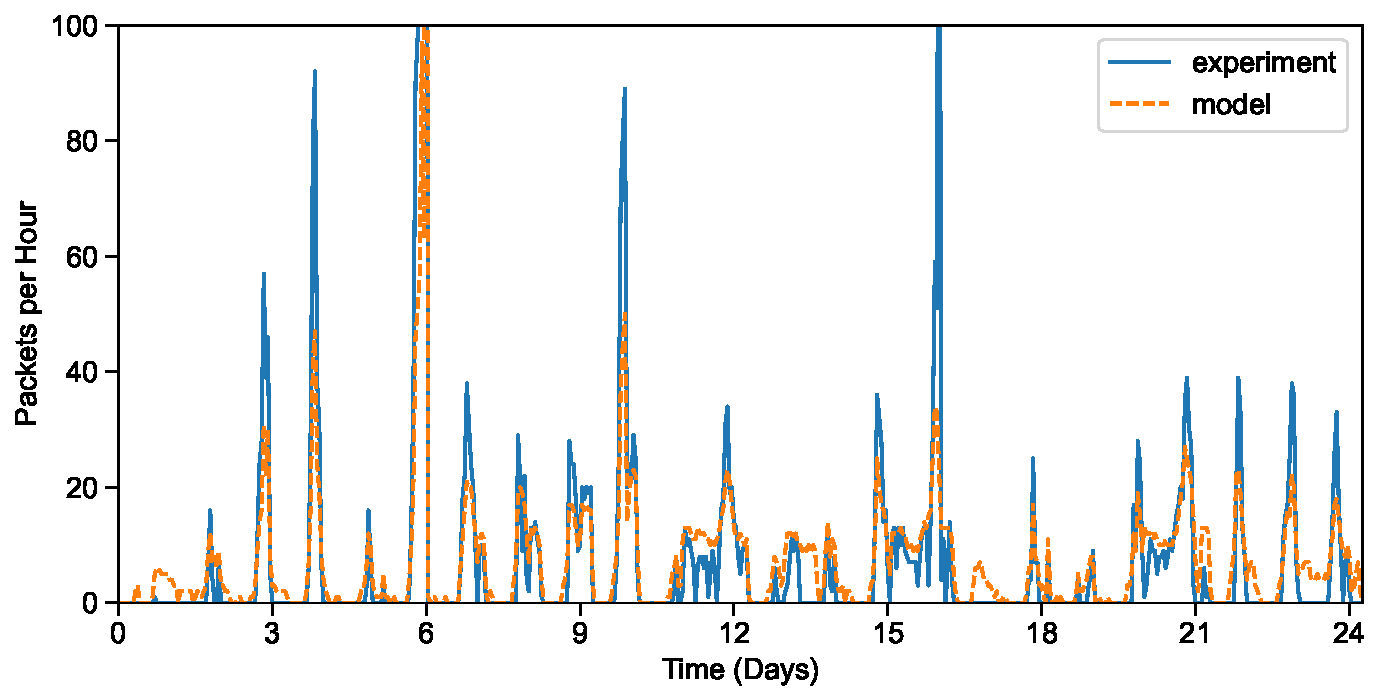
\includegraphics[width=\columnwidth]{figs/capacity/experiment_pkt/exp_vs_sim_pkt}
    \label{fig:eval:pkt}
    \caption{Performance comparison of model expectation versus real batteryless system. 
    Data from a three month deployment of two systems is used to verify our model.
    We use three weeks of illuminance measurements %from a month-long deployment
    to estimate irradiance and model the number of packets transmitted by an
    batteryless node. Average daily error is 15\%, with a standard deviation
    of 17\%. 
    } 
\end{definefigure}

\begin{definefigure}{fig:impl:eval_soc}
    \centering
    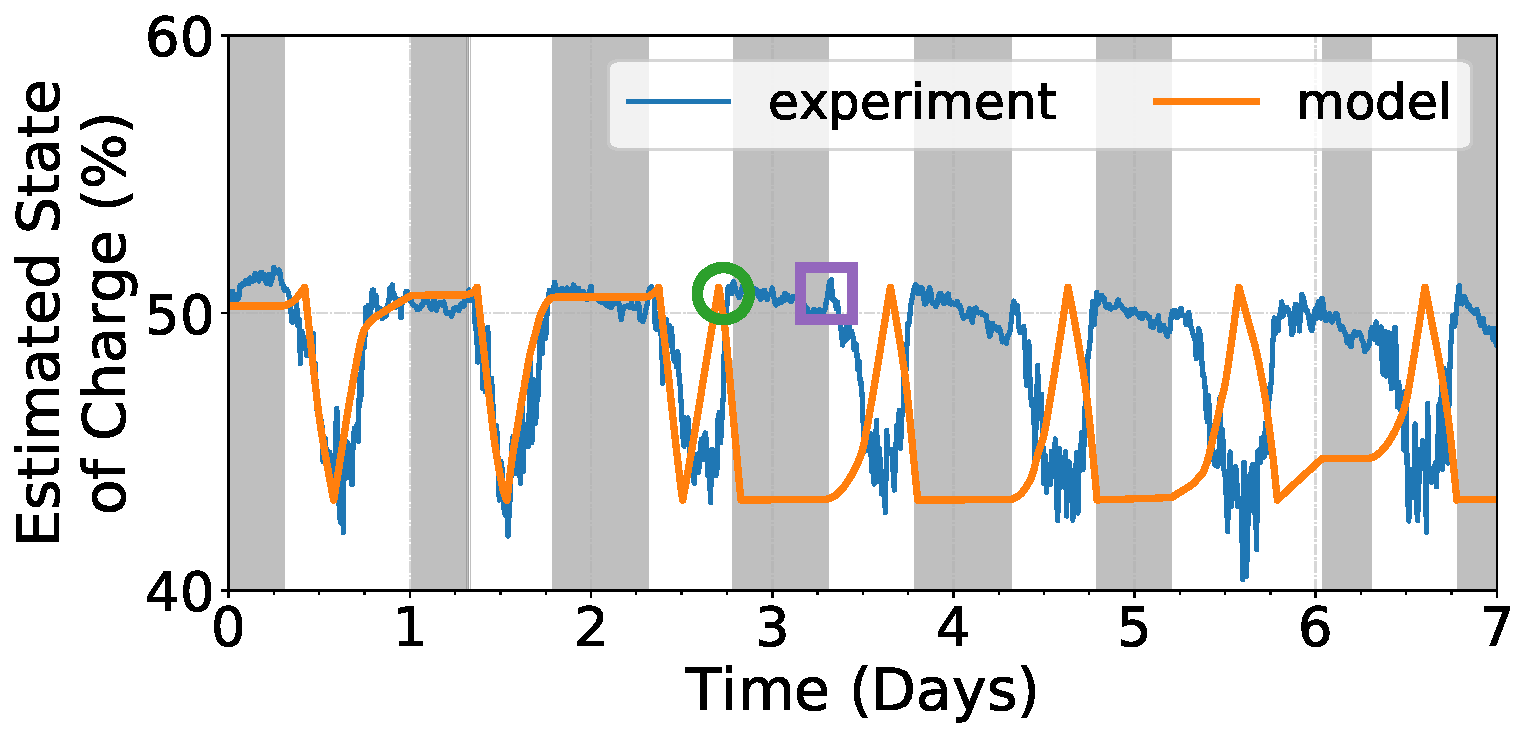
\includegraphics[width=\columnwidth]{figs/capacity/experiment_soc/exp_vs_sim_soc}
    \label{fig:eval:soc}
    \caption{The estimated state of charge of a week of a workload compared to our model's estimation.
    We use three weeks of illuminance measurements %from a month-long deployment
    to estimate irradiance and model the number of packets transmitted by an
    batteryless node. Average daily error is 15\%, with a standard deviation
    of 17\%. (b) We model and measure a \name's state of charge while running a
    ``sense and send'' workload with a 1\,s period for a week, beginning at
    midnight on the first day. Charging hysteresis
    limits of the devices are set at 51\% and 43\%. 
    Shaded regions represent periods of low harvestable potential
    (<\,15\,\textmu W/cm\textsuperscript{2}),
    i.e. nighttime. 
    For the first two days, model predictions
    closely track the experimental measurements. Errors
    in hysteresis and irradiance estimation cause the model to reach its upper
    hysteresis sooner than the experiment does, annotated by the
    \textbf{\textcolor{fig-green}{green circle}}. In actuality, the device
    exits charging hysteresis at the peak marked with the
    \textbf{\textcolor{fig-purple}{purple square}}.
    More importantly, the
    frequency and length of periods spent using harvested
    energy collected in the secondary-cell (downward slopes) are identical.
    %For the batteryless node we see our model
    %underestimate the number of transmitted packets by 10-20\% except for the
    %first day which predicts significantly more packets.  We believe this error
    %is primarily due to a piecewise linear estimation of irradiance from our
    %collected illuminance data, when in reality the relationship is complex and
    %non-linear.  For (b) we estimate the state of charge of \name
    %based on the secondary
    %cell voltage. Differences between the estimated state of charge and the
    %modeled state of charge are primarily due to inflated voltage during
    %charging and voltage droop and bounce back when \name
    %draws current from the secondary-cell.
    %Even though estimated state of
    %charge is not accurate due to this voltage swing, it is clear that the
    %timing of charge and discharge aligns between the model and the
    %experimental data.
    }
\end{definefigure}

\begin{definefigure}{fig:evalcmp}
    \centering
    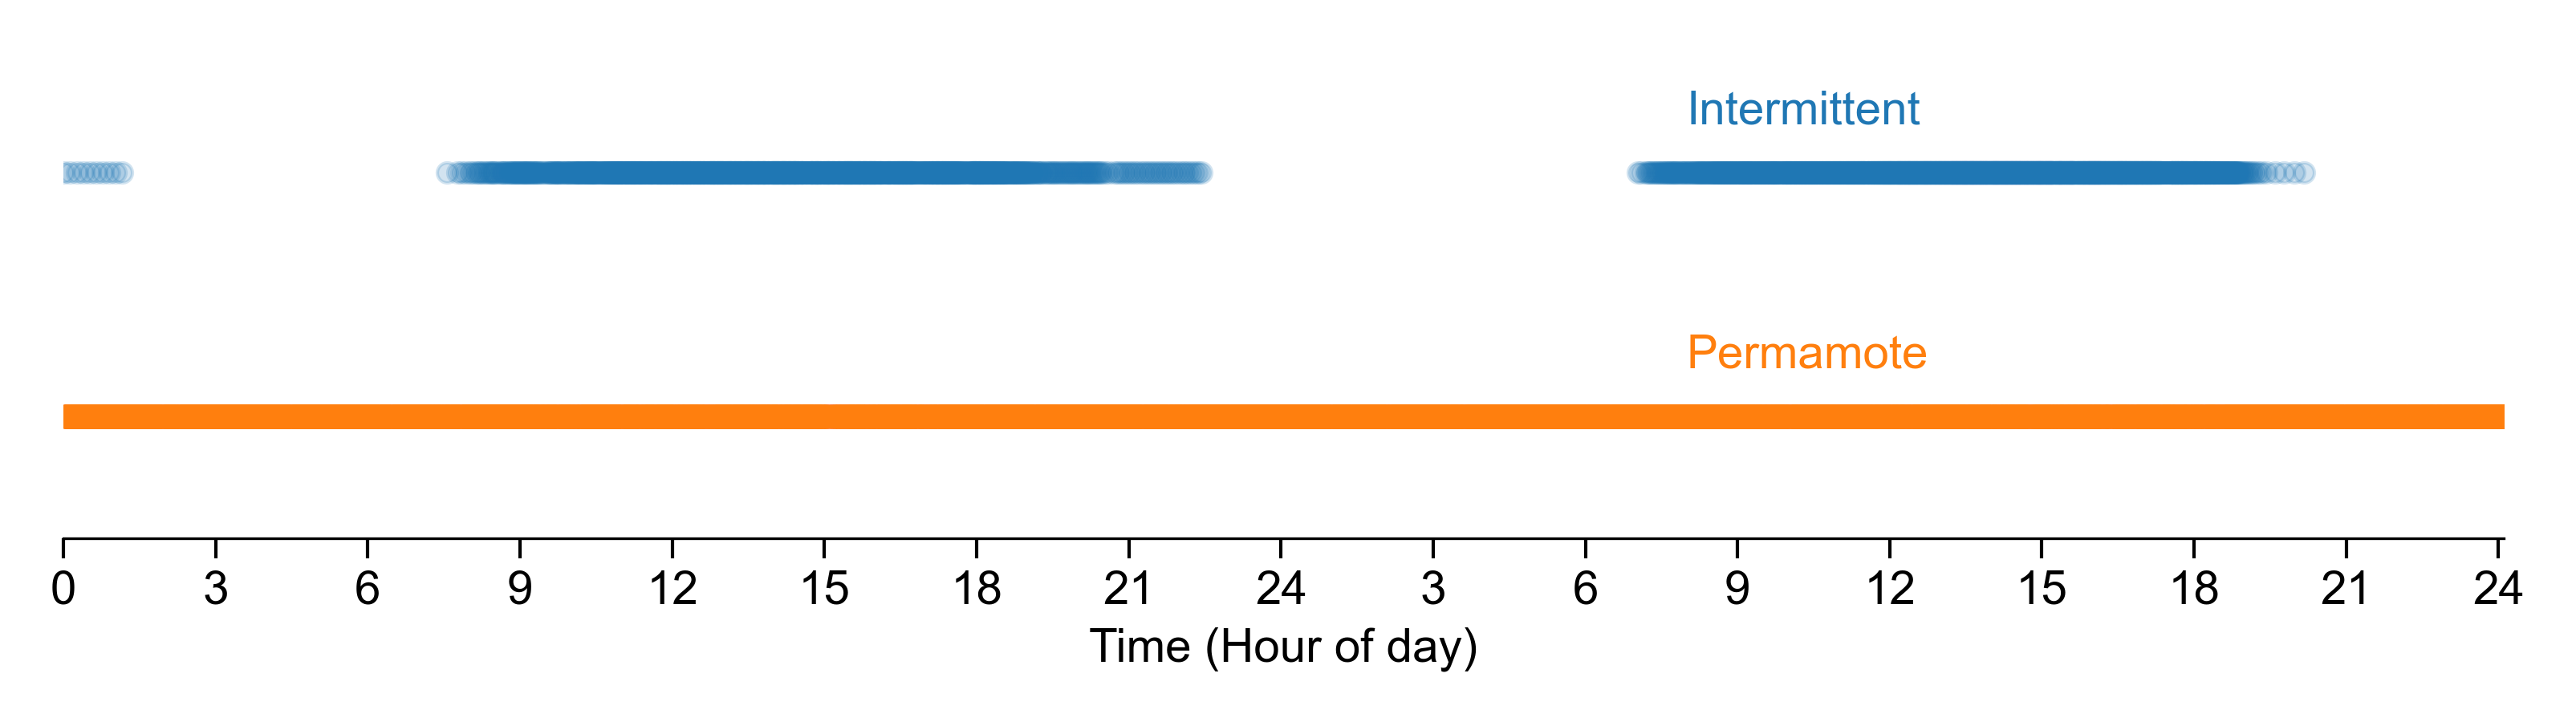
\includegraphics[width=\linewidth]{figs/capacity/experiment_sys_compare/exp_packets_recv}
    \caption{
      \normalfont
        Packets received over two days.
      This figure compares the availability of an
      batteryless design and \name. \name sends a packet every second and does
      so without fail, while the batteryless system is only able to send when
      light is available.
      %This results in periods at night where the
      %batteryless device does not harvest enough energy to sustain operation.
      }
\end{definefigure}

\begin{definefigure}{fig:impl:permamote_life}
    \centering
    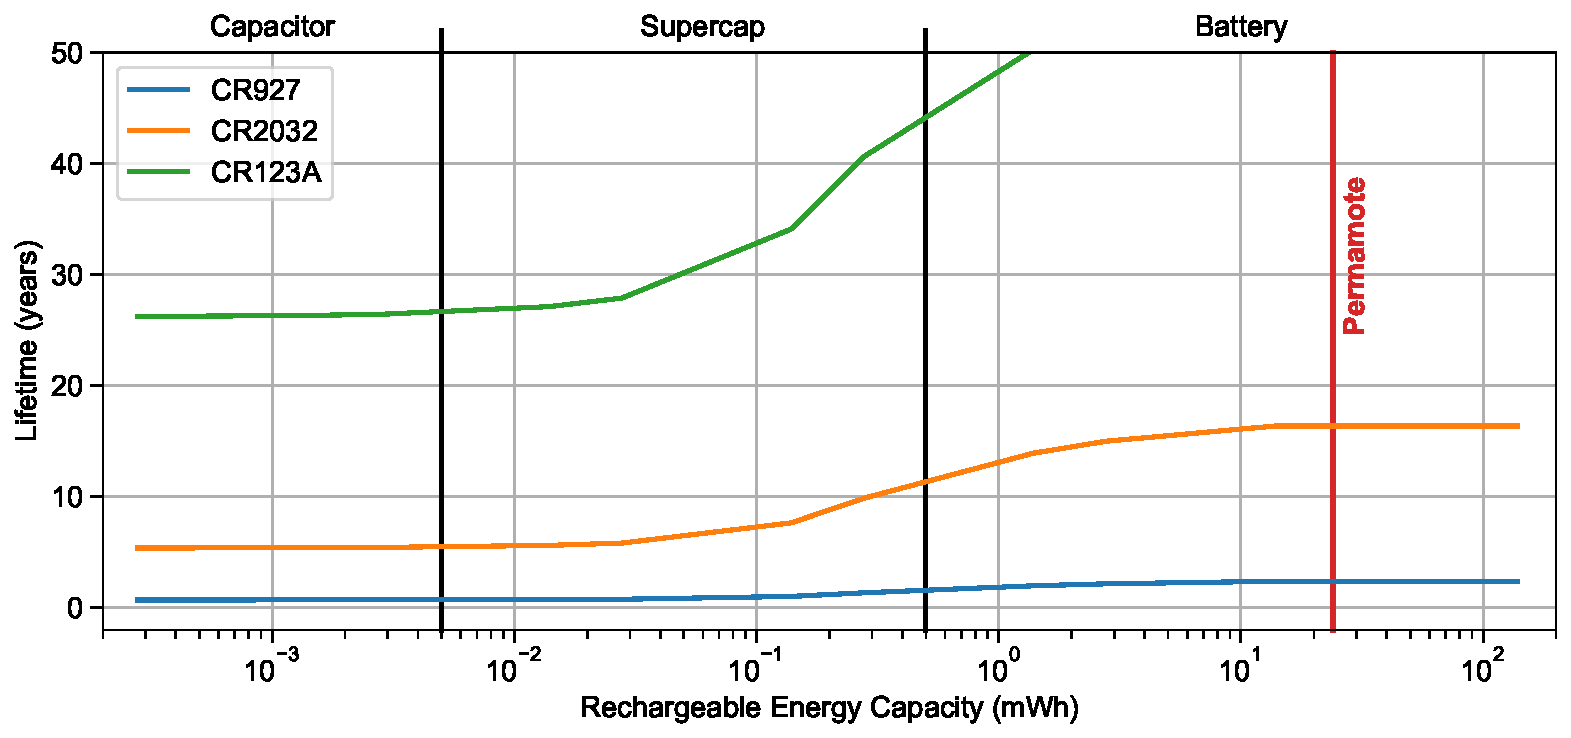
\includegraphics[width=\linewidth]{figs/capacity/primary/sense_and_send_life_vs_sec_size_permamote.pdf}
    \caption{
        Lifetime estimation of the \name sense and send workload given different rechargeable buffer sizes and different primary cell sizes. This figure utilizes the low irradiance Setup A environment and the 30 second sense and send workload period.
      This is a different presentation of \cref{fig:capacity:primary} that identifies the rechargeable capacity of \name with a red vertical line.
      }
    
\end{definefigure}

\begin{definetable*}{tab:related}
  \begin{threeparttable}
  \centering
  \begin{tabularx}{\columnwidth}{@{\extracolsep{\fill}} l | c c| c c| r}
      \thead[l]{Platform} & \multicolumn{2}{c}{\thead{Successful Events\,(\%)}} & \multicolumn{2}{c}{\thead{Long-Running\\Time to Completion Ratio}} & \thead[r]{Lifetime\\(yrs)}\\
                              & Periodic     & Reactive                     & Average & 95th Percentile & \\
    \hline
    Telos \cite{polastre2005telos}                      & 100   & 100   & 1     & 1     & 8.55\\
    Hamilton \cite{kim2018system}                & 100   & 100   & 1     & 1     & 6.75\\
    BLEES \cite{adkins2015michigan}                     & 100   & 100   & 1     & 1     & 1.11\\
    Gecko \cite{yervaGrafting12}                 & 39.5  & 64.9  & 387   & 981   & $\infty$\,\tnote{g} \\
    Capybara~\cite{colinReconfigurable18}\,\tnote{a}    & 46.3  & 72.8  & 37.6  & 1     & $\infty$\,\tnote{g}\\
    Capybara~\cite{colinReconfigurable18}\,\tnote{b}    & 41.1  & 67.1  & 2730  & 8900 & $\infty$\,\tnote{g}\\
    Flicker \cite{hesterFlicker17}                      & 39.3  & 64.2  & 1307  & 5670 & $\infty$\,\tnote{g}\\
    EnHANTs \cite{margolies2015energy}                  & 79.4  & 96.0  & 1     & 1     & \textemdash\,\tnote{h}\\
    DoubleDip \cite{martin2012doubledip}                & 77.9  & 66.5  & 1     & 1     & \textemdash\,\tnote{h}\\
    \cite{raisigel2010autonomous}                       & 78.4  & 66.9  & 1     & 1     & \textemdash\,\tnote{h}\\
    \textbf{\name}\,\tnote{c}                           & 81.2  & 98.3  & 1     & 1     & \textemdash\,\tnote{i}\\
    \textbf{\name}\,\tnote{d}                           & 100   & 100   & 1     & 1     &  35.8\\
    \textbf{\name}\,\tnote{e}                           & 100   & 100   & 1     & 1     &  30.2\\
    \textbf{\name}\,\tnote{f}                           & 100   & 100   & 1     & 1     &  6.27\\
  \end{tabularx}
    \begin{tablenotes}[para]
      \item[a] With capacitors: 400\,\ssi{\micro\farad} ceramic + 330\,\ssi{\micro\farad} tantalum + 67.5\,mF supercapacitor.
      \item[b] With capacitors: 300\,\ssi{\micro\farad} ceramic + 1100\,\ssi{\micro\farad} tantalum + 7.5\,mF supercapacitor.
      \item[c] No primary-cell.
      \item[d] AA primary-cells like Telos.
      \item[e] CR123A primary-cell like Hamilton.
      \item[f] CR2032 like BLEES.
      \item[g] Lifetimes are theoretically infinite for capacitor-based systems.
      \item[h] Not enough information to predict cycling failure time for theses systems.
      \item[i] Expect cycling degradation in 20-50 years, but do not attempt to estimate.
    \end{tablenotes}
  \end{threeparttable}
  \caption{
  \normalfont
      Simulated performance of energy-harvesting systems performing the same workloads.
    For each  platform considered, we model the performance of its energy storage
    architecture. Periodic workload and lifetime estimates are based on a 10\,s
    period, and the reactive workload is scaled to
    generate a maximum of 2000 events per hour (3.4\,s average daily period). 
    \name is the only energy harvesting platform that can provide 100\% availability, while also offering a lifetime of more than triple that of similar battery-only platforms.
    }
\end{definetable*}

\section{Image-based Occupancy Detection}
Besides the utilization of LED lighting and daylighting, another way to increase lighting efficiency in buildings is to automate lighting power states based on human occupancy.
Human occupancy is also a useful metric for regulating building heating and cooling.
The presence and number of people in a space directly effects the amount of heating, ventilation, and air conditioning (HVAC) a building must perform to maintain a temperature set point~\cite{wei2020deep}.
Compared to lighting, building HVAC is much more energy intensive, with cooling consisting of 10\% of the total U.S. electricity consumption in 2021~\cite{aeo2022}. 
Occupancy is measured in lighting control systems, however they often rely on a binary indication of occupancy based on simple ultrasonic or PIR motion detection~\cite{levitonDecora}.
This technique can not quantify the occupancy of a space, and it is prone to false positives and negatives.
Non-human objects that move through a space can trigger an ultrasonic sensor, while any rapid changes in surface temperatures can result in false positives for a PIR sensor.
When a person is not moving sufficiently, both ultrasonic and PIR sensors may sense a false negative.
Instead of, or in addition to these binary occupancy measurements, image sensing can be used to more accurately capture the occupancy, including person count, of a space.
Image inference, including classification and object detection, has been one of the most active areas of modern computer science and machine learning research. 
However, due to the cost and difficulty of deploying wired cameras, long-lived applications based on continuous image sensing has traditionally been untenable.
This is especially true for indoor building-centric applications, where camera density must be higher for sufficient coverage and lifetime must be sufficient to avoid frequent maintenance.

\subsection{Related Work}
Indoor wireless camera sensors have been heavily researched and commercialized over the past fifteen years, but due to the technology available at the time, as well as incompatibilities between design decisions and longevity, these platforms are typically limited to lifetimes of at most weeks to months~\cite{rowe2007firefly,rahimi2005cyclops,blinkindoor,wyzeoutdoor,josephson2019wireless}. 
Deployment of these platforms beyond small or temporary installations remain a challenge due to the cost of frequent battery replacement.
%With the confluence of new and improved COTS technology, like low power processors, radios, and image sensors, it is worth revisiting the design of wireless camera sensors. 

Modern image sensing platforms have taken advantage of technology improvements, as well as employed new techniques to reduce transmit power and increase (or abolish) lifetime. WISPCam~\cite{naderiparizi2015wispcam}, is a battery-free camera that utilizes RFID for power and backscatter communication. It can capture an image every 15 minutes when an RFID reader is 5 meters away. BackCam~\cite{josephson2019wireless} is  another camera platform that utilizes backscatter for communication, but over commodity WiFi. BackCam can stream video at 4 frames per second for a lifetime of 32 days. Similar to WISPCam, BackCam also requires a nearby wall-powered transmitter to generate excitation packets for backscatter communication. Camaroptera~\cite{nardello2019camaroptera} is another batteryless platform, focused on wide-area image sensing. 
The platform uses a long-range LoRa radio and harvests energy from solar panels. It performs local inference to detect people within captured photos and can achieve an end-to-end latency of less than 20 seconds in well-lit outdoor environments. Commercial platforms like the Blink Indoor wireless security camera~\cite{blinkindoor} and the Wyze outdoor camera~\cite{wyzeoutdoor} utilize low power motion detection to minimize energy usage. The Blink Indoor claims a 2 year lifetime consisting of 40000 seconds of recording 720p video on two AA batteries. Wyze estimates a lifetime of three to six months on its internal 5.2\,Ah battery if capturing 10 to 20 video clips per day.

While these modern platforms push the envelop for video streaming or batteryless imaging, they have drawbacks that limit their deployability in indoor spaces. Backscatter-based systems require a nearby carrier transmitter to communicate. Even with a dedicated, nearby transmitter, WISPCam can only periodically capture images every 15 minutes. Camaroptera is designed for outdoor use, and it is unclear if it can capture and send images indoors, especially as its energy harvesting system requires 197\,\uW when idle. 
The Blink camera lasts two years if it is placed in locations infrequently occupied by people. Placing the camera in a kitchen that sees an average 26\% occupancy on weekdays leads to a lifetime of only 1.78 days \cite{josephson2019wireless}. The Wyze camera faces a similar fate if placed in a frequently occupied area.

Image sensing platforms developed by industry and in research exhibit the same design disconnect that we noted in \cref{chap:background}. Commercial image sensing systems largely utilize batteries and avoid energy harvesting, while modern research systems are largely energy harvesting and batteryless.
These two different design result in a deceptive choice between reliable operation with a preallocated energy source but a limited lifetime, or an unlimited but unreliable lifetime with batteryless energy harvesting.
Neither option is satisfactory for many applications, including our indoor human occupancy detection example application that simultaneously demands a long sensor lifetime and high availability.

\subsection{The Performance of a Batteryless Image Sensor}
In this dissertation, we have argued that a batteryless approach is not appropriate for applications with QoS requirements. Designers of batteryless systems rarely evaluate their platforms and frameworks in regards to availability and reliability. However, utilizing the heuristics and simulation tools we have developed in \cref{chap:intuition,chap:capacity}, we can estimate the performance of these systems and identify alternate design decisions that may result in a more performant image sensing system.

In this section, we consider the design and performance of Camaroptera, a batteryless image sensor
~\cite{nardello2019camaroptera,desai2022camaroptera}.
We capture the design details of Camaroptera and use them to simulate the system and examine its performance.
Camaroptera is designed as a primarily outdoor system, and utilizes LoRa for communication and image backhaul.
It performs local inference to detect people in captured frames. A positive detection results in transmitting an image, and if no person is detected, it discards the captured image to preserve energy. 
It harvests solar energy with four small high-efficiency (20\%) monocrystaline solar panels (6.2\ssi{\centi\meter\squared} total area).  Camaroptera stores harvested energy in a 33\ssi{\milli\farad} supercapacitor.
Camaroptera, like many batteryless systems, operates opportunistically. 
Whenever its capacitor is charged sufficiently, it turns on and  performs its workload. 
Camaroptera's workload consists of capturing an image, performing some computations and inference on this image, compressing the image, and finally transmitting the packetized image. 
Camaroptera's energy storage is sized to support the most energy intensive operation in its workload: transmitting a single LoRa packet.
A single packet can not fit an entire compressed image, so Camaroptera relies on multiple power cycles to send between seven and eight packets to transmit an entire image.
All combined, a single image capture and transmission requires 781\ssi{\milli\joule}\footnote{Capture energy: 3.06 (capture) + 0.253 (difference) + 66 (inference) + 40 (JPEG) + 96$\times$7 (transmission) = 781\ssi{\milli\joule}~\cite{desai2022camaroptera}}.
When idle, Camaroptera's power subsystem consumes 197\ssi{\micro\watt}.
With this information, along with operation timing provided by the authors~\cite{desai2022camaroptera}, we are able to complete a simulation configuration like \cref{tab:capacity:parameters} for Camaroptera's hardware design and workload.

For energy income, we synthesize an outdoor irradiance trace based on the EnHANTs Setup D trace. 
The authors evaluated Camaroptera from 5--95\ssi{\kilo\lux}, which roughly corresponds to 4--77\ssi[per-mode=symbol]{\milli\watt\per\centi\meter\squared} for natural light\footnote{For natural sunlight: 1\ssi[per-mode=symbol]{\watt\per\meter\squared} $\approx$ 
122\ssi{\lux}~\cite{michael2020conversion}}.
We scale the mean of the synthesized outdoor trace to represent 10 and 50\ssi[per-mode=symbol]{\milli\watt\per\centi\meter\squared} for an estimate of outdoor irradiance on the same scale.
The simulation results of Camaroptera's average packet distribution under these two harvesting conditions are summarized by \cref{fig:impl:camaroptera_pkt}.
With either income, Camaroptera is able to maintain high image capture and transmit rates when light is available. 
However, as expected of a batteryless system, when light is unavailable, Camaroptera is unable to capture and send many images.
Since Camaroptera performs its workload in response to its energy storage state, it can not maintain a periodic schedule or reliably react and detect the presence of people.

\placefigure{fig:impl:camaroptera_pkt}

This limitation is primarily due to the energy capacity available to the platform. The available energy in an outdoor setting is essentially limitless to a low power embedded system like Camaroptera. 
For the two simulations we consider, our simulated Camaroptera with its capacitor energy buffer is only able to capture 48\% and 21\% of the available energy for the 10 and 50\ssi[per-mode=symbol]{\milli\watt\per\centi\meter\squared} traces, respectively. 
Due to its designed energy capacity, Camaroptera is simultaneously limited in the amount of energy it can capture and the amount of instantaneous energy available to it at any given time.
Given the design heuristics developed in \cref{chap:intuition}, we can determine an estimate for Camaroptera's average income and average workload power if we assume a fixed sensing period instead of the opportunistic operation of the actual platform.
From these averages and using the capacity sizing heuristics from \cref{sec:intuition:capacity}, we can determine an estimate for the minimum sufficient capacity to sustain this workload given our synthesized incomes.
As mentioned earlier, each Camaroptera activation requires 781\ssi{\milli\joule} over 40 seconds, assuming all images go through the entire inference pipeline. The platform's idle power is 197\ssi{\micro\watt}.
While the platform is capable of transmitting an image every 45 seconds to two minutes depending on lighting conditions, we assume a relaxed periodic rate of capturing and transmitting an image every five minutes.
This results in a 2.8\ssi{\milli\watt} average workload power\footnote{~$\frac{781\si{\milli\joule} + (197\ssi{\micro\watt} \times (300 - 40)\si{\second})}{300\si{\second}} = 2.77\si{\milli\watt}$}.

\placefigure{fig:impl:cam_sweep}
From this example workload and Camaroptera's income, we can use the huristics developed in \cref{chap:intuition} to determine the proper capacity sizing for the platform.
With Camaroptera's designed solar panel size, maximum power point voltage, and efficiency, 
it can expect between 12.3 and 61.6\ssi{\milli\watt} average income power from our two synthesized traces.
On average, this theoretical energy income should be more than sufficient to power this periodic sense and send workload, assuming the platform has enough capacity to capture it.
The lower end of this income corresponds to an income margin of over 300\%. 
Considering the sizing factor for income resembling the distribution of Setup D, determined in \cref{sec:intuition:margin}, we should expect a minimum sufficient capacity that is \num{1.4E3} times Camaroptera's workload power. 
This corresponds to an energy capacity of 3920\ssi{\milli\Wh}. 
The 33\ssi{\milli\farad} supercapacitor on Camaroptera only provides 41\ssi{\micro\Wh}. This capacity represents five orders of magnitude less than the minimum sufficient energy capacity predicted by our heuristic.
To further explore the impact of capacity sizing for Camaroptera, we simulate the platform with a sweep of different amounts of rechargeable capacity. 
We change our simulated Camaroptera's workload behavior from an opportunistic strategy to the periodic schedule discussed above.
We sweep capacity from the size of Camaroptera's original energy capacity to the amount predicted by our sizing heuristic.
The results of the simulated platform performance versus capacity are presented in \cref{fig:impl:cam_sweep}.
For each successive simulation that increases energy capacity, the periodic Camaroptera workload is able to achieve higher availability.
With an energy capacity above 100\ssi{\milli\watt\hour}, simulations with the 50\ssi[per-mode=symbol]{\milli\watt\per\centi\meter\squared} income are able to achieve near 100\% availability, while it requires at least 1000\ssi{\milli\watt\hour} for the 10\ssi[per-mode=symbol]{\milli\watt\per\centi\meter\squared} simulations to achieve similar levels of availability. 
Both of these simulation results suggest less energy capacity is required than the previously estimated 3920\ssi{\milli\Wh}.
This is for the same reason as explained in \cref{sec:impl:permamote}: the simulation begins with a partially charged energy buffer to mimic how a real system would be deployed while the heuristic analysis assumes starting from empty.
Thus, the heuristic provides a more conservative estimate that is more likely to result in energy neutral operation over longer periods of time.

Camaroptera was implemented with an energy capacity that was sized to support its most energy intensive task. This arbitrary design decision results in a minimally feasible design that is fails to fully capture and utilize the 
%more than sufficient 
available harvestable energy.
With significantly more energy capacity, Camaroptera would be able to capture more energy, persist through periods of no harvesting potential, and provide significantly higher availability. 
Based on the capacity requirements determined by this analysis, Camaroptera could be redesigned with a medium-sized rechargeable battery, on the order of 1000\ssi{\Ah}, to achieve the higher performance estimated in \cref{fig:impl:cam_sweep}.

\begin{definefigure}{fig:impl:camaroptera_pkt}
    \centering
    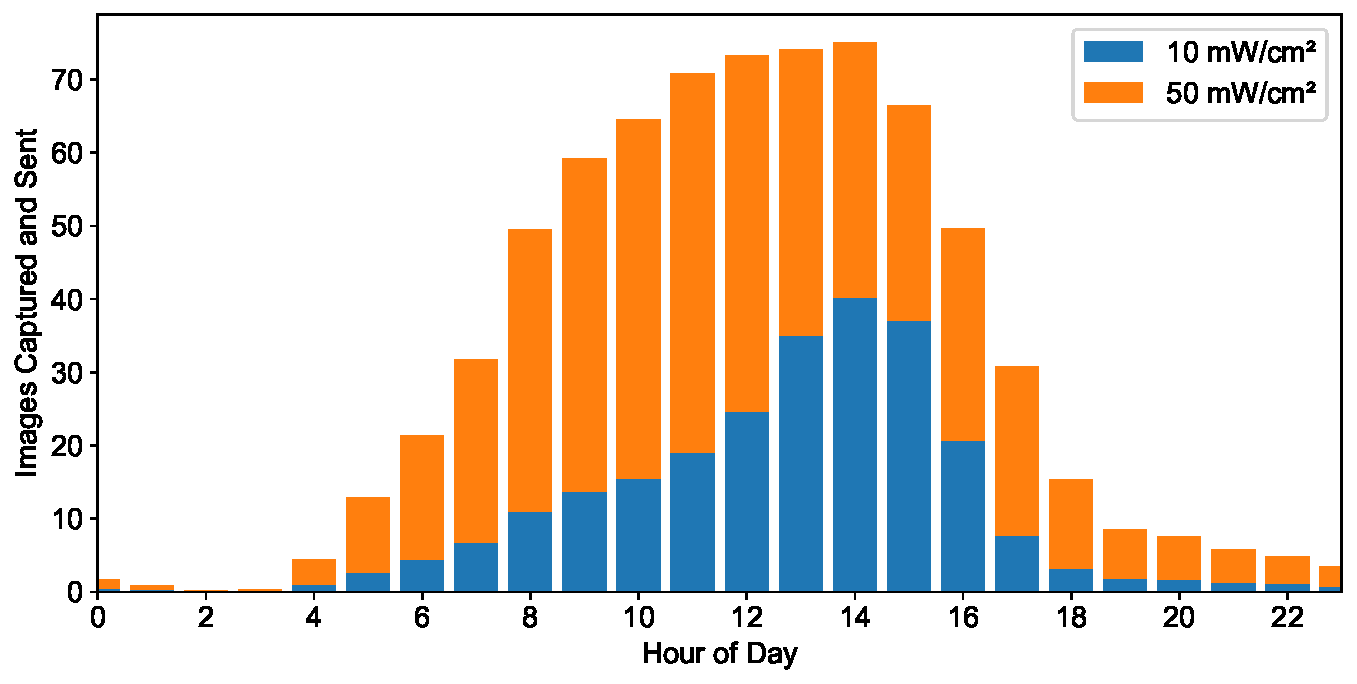
\includegraphics[width=\linewidth]{figs/chap6/camaroptera_performance.pdf}
    \caption{
        The distribution of simulated Camaroptera transmitted image packets per hour in a day. 
        The distribution represents an average over the length of two synthesized outdoor traces (10 and 50\ssi[per-mode=symbol]{\milli\watt\per\centi\meter\squared}) based on the EnHANTs Setup D trace. 
        Camaroptera operation is limited to times when daylight is available, regardless of the scale of average input power. The average number of packets is significantly lower between 6PM and 6AM.
     }
\end{definefigure}

\begin{definefigure}{fig:impl:cam_sweep}
    \centering
    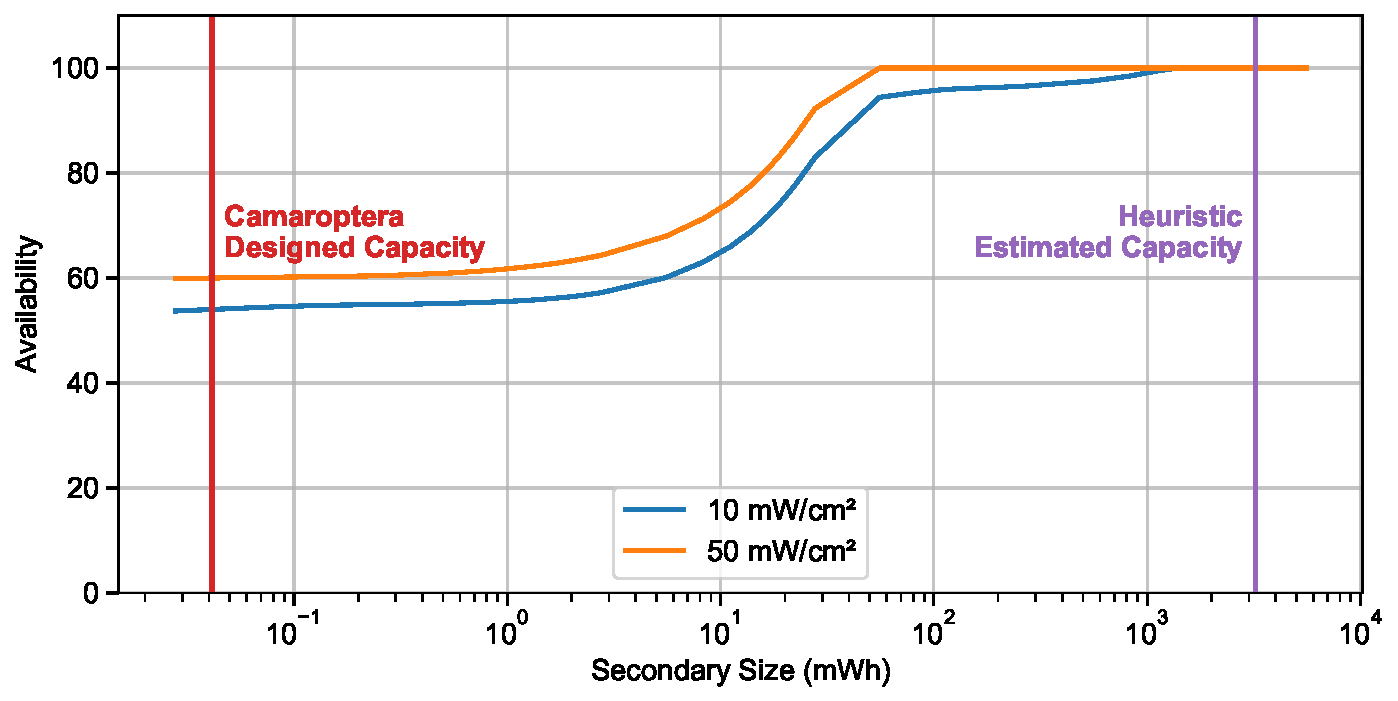
\includegraphics[width=\linewidth]{figs/chap6/camaroptera_simulation.pdf}
    \caption{
        The availability of Camaroptera running a five minute sense and send workload, as energy capacity is increased from that offered by its original 33\ssi{\milli\farad} supercapacitor to the minimum sufficient capacity estimated by the heuristics developed in \cref{sec:intuition:capacity}.
        Capacity must be increased by five orders of magnitude in order to achieve near 100\% availability.
     }
\end{definefigure}

\subsection{The Design of an Indoor Wireless Image Sensor}
Due to Camaroptera's relatively high active and idle power requirements, it is unsuitable for use in many indoor environments. 
Designing an image sensor for indoor use will require different design decisions to achieve lower power operation.
An indoor sensor does not need to depend on higher power wide-area communications like LoRa. Instead, with  modest infrastructure investment, an indoor platform can rely on low power personal- or local-area networks.
Besides data transmission efficiency, power efficiency can be improved through the use of a more efficient and capable processor.
Idle power requirements can be reduced through the elimination of Camaroptera's hysteresis circuitry, and instead utilizing simple power gating to reduce component quiescent power. 
Using the heuristics and simulation tools developed, we can also identify the appropriate size of our energy harvesting, buffer capacity, and non-rechargeable storage to maximize energy available to our application. 
The next few sections expand on these design changes for indoor image sensor we name \namec.

\subsubsection{Indoor Wireless}
We design \namec to be untethered from wired communication and power. There are several options we consider for \namec's networking, including WiFi, and personal area networks like BLE and 802.15.4. WiFi is attractive as it supports high bandwidth, which would be appropriate for transmitting large data like images. However, many low power WiFi SoCs like the ESP32 have significant idle and startup power requirements~\cite{esp32}. 
If included on \namec, a WiFi radio or SoC must act as an external, power-gated component to reduce idle current. 
This complicates system design, and it is unclear if WiFi start up cost is worth the bandwidth advantage. 
Instead, we focus on technologies like BLE and networks built on top of 802.15.4. 
These networks are specifically designed to cater to devices that spend the majority of their lifetimes in an ultra low power sleep state. 
We trade off bandwidth and the time to send images for a simpler design and lower overall power.
 
%We utilize 6LoWPAN to enable a modern, IP-enabled design that allows direct end-to-end communication between sensors and the desired endpoint. We design a low power end-to-end image transfer architecture that makes images captured by \name{} easily accessible in high level languages and machine learning frameworks.
%To reduce the energy and time required to send images, \name{} compresses each image captured before transmission. 
%The use of IPv6 enables \name{} devices to directly send images to endpoints without any custom application layers. Received images can then be used for inference or published on a data stream.

\subsubsection{Processor Selection}
Processing and manipulating images requires significant computing and memory resources when compared to sensor data with lesser dimensionality, like periodic illuminance and color sensor data that is collected by \name.
Camaroptera's 16--bit, 16\ssi{\mega\hertz} processor requires 25 seconds of constant computation to compress a 160$\times$120 JPEG image with floating point emulation, and seven seconds to compress the same image with a fixed point algorithm.
This represents a significant amount of time for a low power device to be active and continuously computing.
The Camaroptera design is severely limited in digital signal processing by its processor selection. 
For \namec, we consider more capable, faster, processors with a 32--bit path and floating point support. 

\subsubsection{Power Supply}
Like \name, to support fully wireless operation for a long lifetime, \namec optimizes energy harvesting and storage through the use of rechargeable and non-rechargeable batteries.
As we have explored previously in our analysis of Camaroptera, vision applications require significant energy to capture images, process them, and transmit them. 
We size \namec's battery in the same manner as \name, utilizing the heuristics and simulation tool from \cref{chap:intuition,chap:capacity} to determine a sufficient capacity.
To determine this, we take benchmarks of capturing and transmitting images over an 802.15.4 network, and utilize these benchmarks to estimate an average power.
We utilize the same indoor irradiance traces that we considered previously.

Indoor energy harvesting is inconsistent and variable, and \namec will operate close to the edge of harvestable power that is reasonably available in many indoor environments.
To augment harvested energy, we include a backup nonrechargable battery on \namec. A backup battery allows continuous operation regardless of energy harvesting conditions. 
It safeguards the system from the volatile nature of energy harvesting, at the cost of a finite, but very long, lifetime.
%For intermittent sensors, this unreliability means the system can lose power at any moment, and any volatile state will be lost. These systems deal with this unreliablity in a number of ways, including techniques like checkpointing~\cite{luciaIntermittent17} and federated or reconfigurable capacitor storage~\cite{hester2017flicker,colin2018reconfigurable}.
%Intermittent capacitor-based systems utilize techniques like checkpointing \cite{luciaIntermittent17}, where the processor saves execution state before running out of power allow these platforms to continue to make forward progress on tasks.  
%However, as their operation is inherently tied on the availability of harvestable energy, they can not maintain any guarantees about reliability. 

\subsubsection{Other Considerations}
\namec includes additional sensors besides a camera to limit duty cycle and minimize idle power. A PIR sensor is used to sense motion, providing an ultra low power wake up mechanism for capturing images. Performing imaging on event detection instead of periodically can save considerable amounts of energy and extend lifetime. The platform also has a light sensor that can interrupt on large changes in light illuminance. This provides another wake up mechanism, allows \namec to detect when it is too dark to capture a useful image, and enables illuminance calibration for captured images. Both PIR and illuminance sensors require many orders of magnitude less energy than an image sensor to sense motion or illuminance.

To address the long-term relevancy of the platform, we also support an over-the-air update mechanism such that \namec can receive regular updates to improve energy management. Additionally, updates can be used to deploy new inference algorithms and models, as well as change image capture workload behavior. The platform can be configured to periodically take pictures, use the low power wake up mechanisms mentioned previously, or use some other software heuristic to only send interesting images.

\subsection{\namec Implementation}
\begin{definefigure}{fig:block}
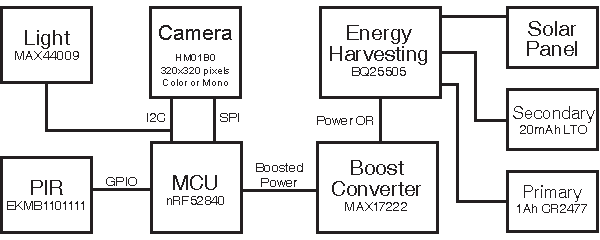
\includegraphics[width=\columnwidth]{figs/permacam/figs/block_diagram.pdf}
\caption{\name system block diagram.
The system is based on the Himax HM01B0 camera and the Nordic NRF52840 MCU. We include a light and PIR sensor to provide a low power wake up mechanism to drive image capture. A hierarchical energy harvesting system with a rechargeable and non-rechargeable battery are utilized to provide a long, reliable lifetime to the system.
}
\end{definefigure}

\begin{definefigure}{fig:arch}
\centering
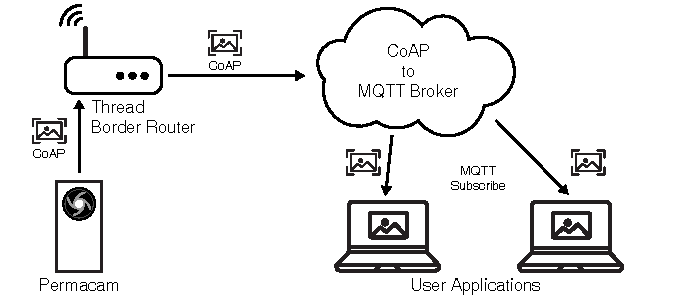
\includegraphics[width=\columnwidth]{figs/permacam/figs/arch.pdf}
\caption{The \namec end-to-end image transfer architecture. \namec uses OpenThread, a 6LoWPAN network. This allows it to transmit images over the CoAP block protocol directly to any IP endpoint. We implement a CoAP server to receive and reassemble image, demosaic them, and publish them over an MQTT stream. This CoAP server can be local to the sensors if privacy is desired. User applications running on PCs or on servers can easily subscribe to incoming images.
}
\end{definefigure}

\begin{definetable}{tab:permacam:components}
    \begin{threeparttable}
        \centering
        \footnotesize
        \begin{tabularx}{\columnwidth}{@{\extracolsep{\fill}} l | l | c | c}
            Component                           & Function                     & Active Current          & Idle Current \\
            \hline
            Himax HM01B0                        & Image sensor                  & 2.0 mA                & 25.1\,\uA\,\tnote{a} \\
            \multirow{2}{*}{Nordic NRF52840}    & Processor                     & 52\,\uA/MHz           & 3.16\,\uA\,\tnote{b}  \\
                                                & Radio                         & 4.8\,mA @ 0\,dbm      & \textemdash\,\tnote{b}\\
            Ambiq AB1815-T3                     & Real time clock               & 55\,nA                & N/A\,\tnote{c}  \\
            Maxim MAX44009                      & Light sensor                  & 650\,nA               & N/A\,\tnote{c}  \\
            Panasonic EKMB11011                 & PIR Occupancy                 & 100\,\uA              & 1\,uA  \\
        \end{tabularx}
    \end{threeparttable}
    \begin{tablenotes}[para]
    \scriptsize
    \item[a] Power gated when not in use.\\
    \item[b] Sleep current for both processor and radio, full RAM retention, wake on low freq. timer.\\
    \item[c] No shutdown or idle mode.
    \end{tablenotes}
    \vspace*{1mm}
    \caption{
    \normalfont
    The components used in \namec, many of which are shared by \name. They represent some of the lowest power options currently available. Due to the extremely low idle power of all included components, \namec is able to sleep at 4.4\uA. 
    }
\end{definetable}

\begin{definefigure}{fig:demosaic}
\centering
\begin{subfigure}{0.49\columnwidth}
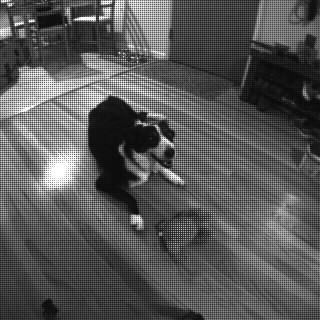
\includegraphics[width=\columnwidth]{figs/permacam/mosaic.jpeg}
\end{subfigure}
%
\begin{subfigure}{0.49\columnwidth}
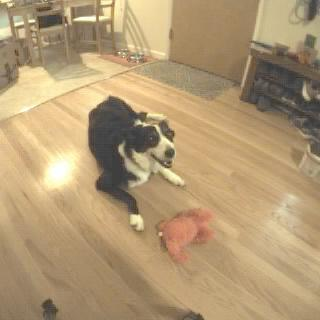
\includegraphics[width=\columnwidth]{figs/permacam/demosaic.jpeg}
\end{subfigure}
\caption{\normalfont{An image from \namec, displayed as a mosaiced image (left) and demosaiced (right).}}
\end{definefigure}

\begin{definetable}{tab:measurements}
\centering
\begin{tabular}{l S[table-format=1.3] S[table-format=2.2]}
{Operation} & {Latency (s)} & {Energy (mJ)} \\
\hline
{Image Capture}           & 1.10  & 4.96\\
{JPEG Compression (Q=90)} & 0.203 & 1.71\\
{Image Transmission}      & 6.67  & 73.8\\
\hline
Total                   & 7.97 & 80.5
\end{tabular}
\caption {
    Latency and energy measurements for key operations on \namec{}, including image capture, compression, and image transmission. Measurements are averaged over 20 images. %An image capture actually consists of multiple frames to calibrate the exposure. We configure \name to wait four frames before capturing an image.
}
\end{definetable}

\begin{definefigure}{fig:impl:permacam_sweep}
\centering
    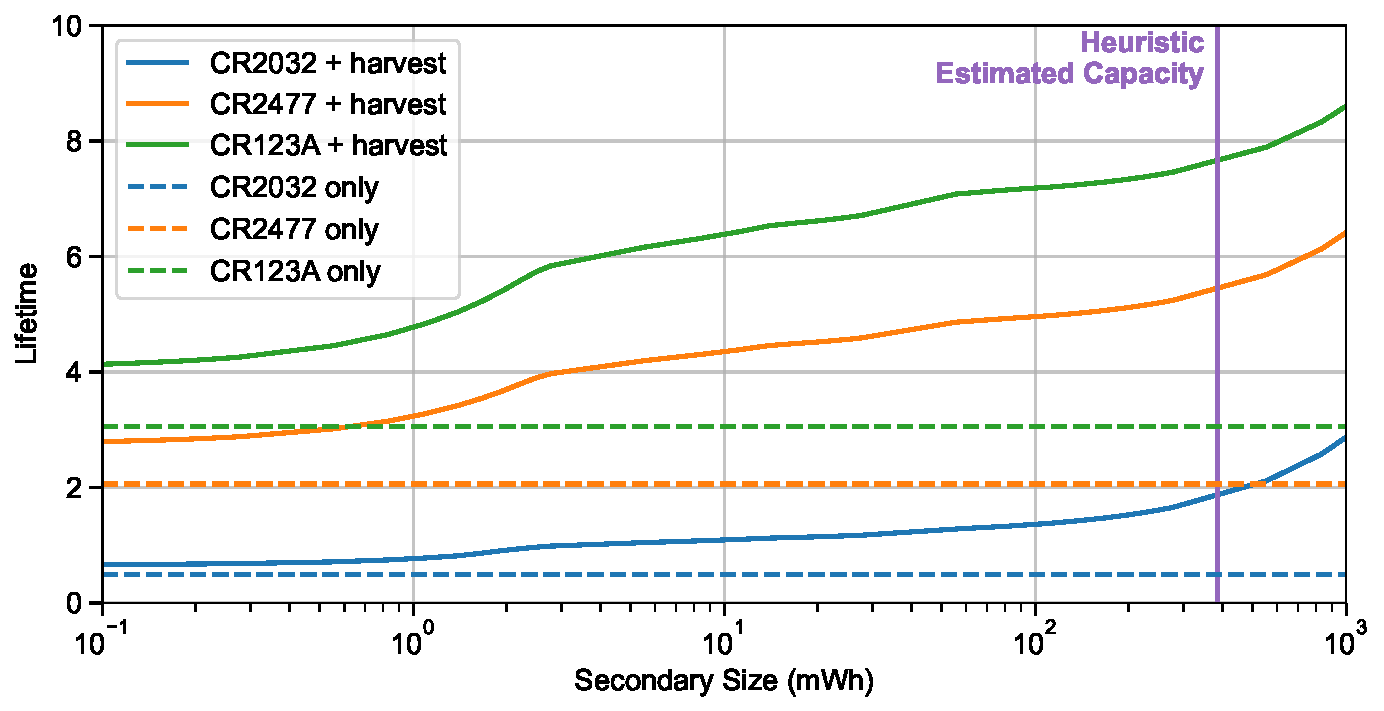
\includegraphics[width=\columnwidth]{figs/chap6/permacam_simulation.pdf}
    \caption{
        Lifetime estimates from \namec simulations with various rechargeable and non-rechargeable energy capacity. The addition of energy harvesting results in capturing more than double the energy provided by a non-rechargeable cell alone. The addition of a CR2477 results in over five years of lifetime for \namec.
    }
\end{definefigure}

In this section, we explore the implementation of \namec{}, including component selection, techniques to enable a low power camera interface, and architectural details about the energy harvesting and storage architecture

\placefigure{fig:block}

We implement the design of \namec{} in an \textbf{open source}
hardware\footnote{\url{https://github.com/lab11/permamote/tree/master/hardware/permacam/rev_a}}
and software\footnote{\url{https://github.com/lab11/permamote/tree/master/software/apps/permacam/camera_coap}}
implementation. The platform is built around the Himax HM01B0 ultra low power camera \cite{hm01b0}. This camera has also enabled other platforms like BackCam \cite{josephson2019wireless} and Camaroptera \cite{nardello2019camaroptera}. The Himax camera is available in two different versions: monochrome and color. 
We use the color version of the sensor to ensure the ability to capture color information of images, but the two versions are pin compatible and can be interchanged. The other key component of the design is the SoC processor. 
For a processor, we select the Nordic nRF52840 Cortex-M4F SoC as it is one of the most power efficient processors available, includes a Floating Point Unit (FPU), and is relatively fast compared to other low power microcontrollers at 64\,MHz. 
An FPU allows the platform to perform floating point dependent tasks like image compression. 
It has a multiprotocol BLE/802.15.4 radio that is well supported by OpenThread, an open source implementation of the Thread 6LoWPAN mesh network protocol~\hl{todo cite}. 
It features comparatively large amounts of flash (1\ssi{\mega\byte}) and SRAM (256\ssi{\mega\byte}), which is enough to capture images and perform some local processing. 
We include an ultra-low power real time clock (RTC) to provide accurate image timestamps. 
The platform also features an ultra low power PIR sensor and illuminance sensor to provide a low power wakeup mechanism and illuminance calibration for captured images. 
A block diagram of the major system components is displayed in \cref{fig:block}. 
Characteristics of the sensors and the MCU are summarized in \cref{tab:permacam:components}. 
In the next few sections we describe \namec{}'s implementation, including the MCU to camera interface, energy harvesting architecture, image compression methods, the end-to-end image transmission architecture, and an implementation of onboard person classification.


\subsubsection{Camera Interface}
The majority of image sensors do not support normal sensor interfaces like I2C or SPI to transfer data. Instead they rely on high frequency ($\geq$8\,MHz) serial or parallel data busses. This is because images are many kilobytes or megabytes in size, and data transfer must be at a high frequency or parallel to transfer multiple frames per second. The majority of embedded processors, the nRF52840 included, are not designed to interface with parallel camera busses. Traditionally, platforms have used intermediate hardware like dedicated processors, CPLDs or FPGAs to interface with image sensors and buffer frames \cite{rowe2007firefly,rahimi2005cyclops}. The Himax HM01B0 has two interfaces, an I2C command interface and a serial, 4x, or 8x data interface.
The Himax HM01B0 requires an input master clock (MCLK) of 3-36\,MHz to drive internal sensor timings and outputs a pixel clock (PCLKO), frame valid (FVLD), and line valid (LVLD) signals \cite{hm01b0}. It can be configured to capture full frame (320x320), QVGA (320x240), and if the mono version of the sensor, downscaled QQVGA (160x120) resolution images. In \namec{} we capture full frame images and use the color version of the sensor. 
This version produces color filter array (CFA) images. 
A CFA is an alternating "mosaic" of green-blue-green and red-green-red rows of pixels~\cite{bayer1976color}. 
Each pixel corresponds to a single color, and through post-processing known as "demosaicing", a three channel RGB image is generated from the single channel representation. 
An example of a mosaiced image and its demosaiced counterpart are displayed in \cref{fig:demosaic}.
\namec{}'s processor does not possess enough memory to locally demosaic an full image so any inference or transmission must be done with the mosaiced image. 
We power-gate the HM01B0 camera on \namec, allowing the system to completely power the camera off and enter the lowest possible power state.

\placefigure{tab:permacam:components}

Other systems that utilize the Himax HM01B0 camera including BackCam, Camaroptera, and the Sparkfun Edge have developed a bitbang protocol to emulate a parallel interface \cite{josephson2019wireless, nardello2019camaroptera, sparkfunedge}. This is possible because their processors support GPIO direct memory access (DMA). This allows the GPIO peripheral to directly write to memory, avoiding costly processor cycles to load GPIO state into registers and then write it to memory. This optimization allows a bitbang protocol on these platforms to operate faster than the HM01B0's minimum operating frequency. However, a bitbang protocol is undesirable because it requires the processor to be on during an image transfer, consuming additional energy. The nRF52840 does not support GPIO DMA. 
Because of this, developing a bitbang protocol that adheres to the required camera timing is infeasible. 
Instead, we note that the camera serial protocol closely resembles SPI, and the nRF52840 implements an 8\,MHz SPI peripheral with DMA support. 
The camera PCLKO signal is identical to SCLK, and can be gated by the LVLD signal. 
The LVLD signal from the camera indicates when a line of the image is being transmitted, and is analogous to a SPI chip select line. However, this line is active high, and most SPI implementations, including the hardware on the nRF52840, expect active low. Inserting a low latency inverter in between the LVLD output of the camera and the MCU allows the nRF52840 SPI peripheral to interface with the camera. 
This has the added benefit of reducing power required to read in images as the processor can sleep while the SPI peripheral directly writes images to memory.

\placefigure{fig:demosaic}

\subsubsection{Image Compression}
To reduce energy and time required to transmit images, we employ JPEG compression on images prior to transmission. We use the Moodstocks JPEC encoder, a simple and portable monochrome JPEG encoder written in C \cite{moodstocks}. JPEG compression, like most DSP algorithms, relies heavily on floating point arithmetic. Due to its integrated FPU, \namec{}'s processor is able to compress full resolution 320x320 images in 210\,ms.
This encoder is also used in Camaroptera \cite{nardello2019camaroptera}, although this platform is based on the MSP430, which lacks an FPU. It requires 25 s to compress an downsampled 160x120 image using floating point emulation, and 7s when JPEC is adapted to fixed point math. This fixed point adaptation also reduces image quality slightly. It is clear that a camera platform like \namec{} benefits greatly from the inclusion of a faster, more capable processor.
JPEG is not designed to compress mosaiced images. However, we find that monochrome compression with a high quality setting does not overly degrade image fidelity or color representation. We explore the effects of monochrome compression on \namec's captured images further in \cref{eval:compression}.

\placefigure{tab:measurements}

\subsubsection{Energy Harvesting and Storage}
The energy storage architecture for \namec{} is built around the TI BQ25505~\cite{bq25505} maximum power point tracking boost converter, like \name. 
The output of the BQ25505's power OR is boosted to the system voltage by a MAX17222 regulator to power all components under a single voltage domain.
We use a 10.9\ssi{\centi\meter\squared} amorpohous photovoltaic to charge a rechargeable LTO battery.
We size this LTO battery according to the capacity heuristic from \cref{sec:intuition:capacity}.
The \namec workload consists of an image capture, JPEG compression, and image transfer. These operations are benchmarked on the nRF52840 SoC and HM01B0 image sensor and summarized in \cref{tab:measurements}.
If we assume a periodic workload, capturing, compressing (at JPEG quality 90), and transmitting an image very ten minutes, \namec will require 148\ssi{\micro\watt} on average\footnote{~$\frac{80.5\ssi{\milli\joule} + 14.5\ssi{\micro\watt}\times(600-7.97)}{600}$}.
This workload for \namec is pushing the bound on the energy that is harvestable within an indoor environment. 
If we consider there is no harvesting margin, this suggests a minimum sufficient capacity on the order of \ssi{\milli\Wh}. 
This capacity corresponds closely to a 125\ssi{\milli\Ah} LTO battery with a nominal 2.4\ssi{\volt}, which is the closest size available for purchase.
We simulate \namec's workload under the conditions of EnHANTs Setups A and D, while sweeping capacity and considering several different sizes of backup batteries.
From the results, presented in \cref{fig:impl:permacam_sweep}, we can determine an appropriate backup battery size to achieve an acceptable lifetime.
We select a lithium 3\ssi{\volt}, 1\ssi{\Ah} CR2477 coin cell battery. This amount of backup energy results in a design that can persist more than five years while capturing an image every ten minutes.
\placefigure{fig:impl:permacam_sweep}


\subsubsection{End-to-end Image Pipeline}
To support transmitting full images, we implement a full application stack based on standard IP-based protocols. This end-to-end image architecture is depicted in \cref{fig:arch}.
We choose to use OpenThread, an open source implementation of the Thread network protocol for \namec devices. Thread is a 6LoWPAN mesh network, and allows packets to be sent end-to-end over a standard IP network. OpenThread also provides implementations of useful protocols like CoAP, SNTP, and DNS. 
CoAP is a lightweight restful protocol similar to HTTP, but over UDP \cite{shelby2014constrained}. 
On top of OpenThread's CoAP API, we implement the CoAP Block add-on feature. This allows us to fragment large data like an image across multiple CoAP payloads \cite{bormann2016block}. 
The choice to use CoAP block is a reluctant one however, and was based on the available implementations of reliable transfer protocols for low power networks.
\namec image transmission is a perfect application for TCP, although TCP is rarely implemented for low power networks. TCP has been shown to be provide a 40\% higher throughput compared to CoAP block over an OpenThread network~\cite{kumar2020performant} over an OpenThread network. However, TCP was not implemented in the version of OpenThread used during the implementation of \namec, limiting us to CoAP block.

\placefigure{fig:arch}

\namec captures an image, compresses it using JPEG, and transmits the image using a CoAP blockwise transfer. The CoAP block messages are sent to an endpoint that reassembles them, parses their contents, and publishes a JSON message over an MQTT broker. An application running on the endpoint listens for the transmitted mosaiced images, demosaics them, and republishes the color image for application use. High level applications wishing to interface with images captured by \namec devices simply must subscribe to the relevant device topics to receive images. From there, the images can be easily processed in frameworks like OpenCV, Tensorflow, or Pytorch~\cite{tensorflow2015-whitepaper, pytorch,itseez2015opencv}.

In addition to our data backhaul pipeline, we implement an independent update server. \namec devices arbitrarily poll the update server every 24 hours for a new application image. If a newer image exists, it downloads it over a CoAP blockwise transfer and applies it. This allows users to deploy new applications quickly across an entire deployment with minimal intervention.

\subsubsection{Local Image Classification}
In addition to transmitting images, we also demonstrate the ability of the platform to perform local inference.
While performing local object detection is not feasible with the memory and compute constraints of \namec,image classification (with a limited number of classes) is not. 
To explore the capabilities of machine learning inference on \namec,
we modify and train our own MobileNets v1 network to perform person classification. We then deploy it to \namec's processor using TensorFlow Lite for Microcontrollers. 

The parameter flexibility of MobileNets v1 allows us to reduce the size of the model so it can fit on a microcontroller. We reduce the size of the network by reducing the depth of each convolutional layer by 75\% ($\alpha$ = .25).  
%\hl{cut some of model details if space needed: }
The model consists of a regular convolution with batch normalization followed by multiple depthwise separable convolutions~\cite{howard2017mobilenets}. 
%The result of the convolutions is passed through an average pooling layer and a dense layer of 2 units, resulting in a person and no person score. A kernel size of 3 is throughout all convolutions.
There is insufficient memory to perform the forward pass on full sized 320x320 images, so images need to be downscaled. We configure this network for different input image dimensions including 48, 72, 96, and 120.
We train this model for 80 epochs on the Visual Wake Word dataset~\cite{chowdhery2019visual} to achieve a validation accuracy of 78\%, compared to a 90\% accuracy with an unmodified MobileNet. The model weights require 230\.kB after post-training quantization and achieve an accuracy of 76\% for input images of size 120x120 when using TensorFlow in Python. We deploy this model on \namec and evaluate its performance in \cref{eval:localinf}.

\subsection{\namec Evaluation}
\hl{TODO: need to go through this section and edit + fix figures}



\begin{definefigure}{fig:compression}
\captionsetup[subfigure]{labelformat=empty}
\centering
\begin{subfigure}{0.4\columnwidth}
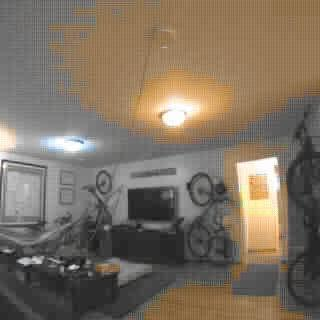
\includegraphics[width=\linewidth]{figs/permacam/30.jpeg}
\vspace{-1.5\baselineskip}
\caption{30}
\label{fig:30}
\end{subfigure}
%
\begin{subfigure}{0.4\columnwidth}
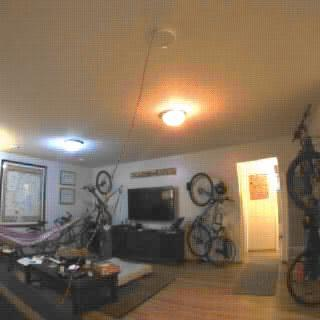
\includegraphics[width=\linewidth]{figs/permacam/70.jpeg}
\vspace{-1.5\baselineskip}
\caption{70}
\label{fig:70}
\end{subfigure}
\par\medskip
\begin{subfigure}{0.4\columnwidth}
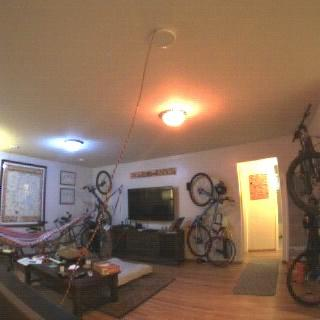
\includegraphics[width=\linewidth]{figs/permacam/93.jpeg}
\vspace{-1.5\baselineskip}
\caption{93}
\label{fig:93}
\end{subfigure}
%
\begin{subfigure}{0.4\columnwidth}
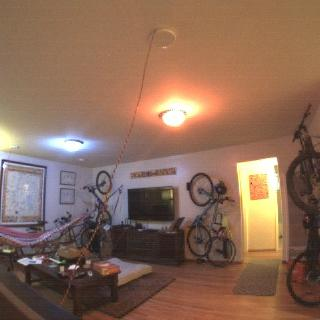
\includegraphics[width=\linewidth]{figs/permacam/raw.jpeg}
\vspace{-1.5\baselineskip}
\caption{raw}
\label{fig:raw}
\end{subfigure}
\caption{An image compressed with different quality factors. \normalfont{In this scene, we set smart lights to bright, intense colors to elucidate the effects of compression on color representation. Compression is performed on the mosaiced version of the image, which after transmission is demosaiced into the color representations displayed. Due to this, an image compressed with a low quality factor loses significant color information compared to the raw image. Luckily, high quality factors produce a near-indistinguishable representation of the raw image. We explore a more quantitative view of image similarity in \cref{fig:ssim}.}}
\end{definefigure}

\begin{definefigure}{fig:size-time-energy}
    \centering
    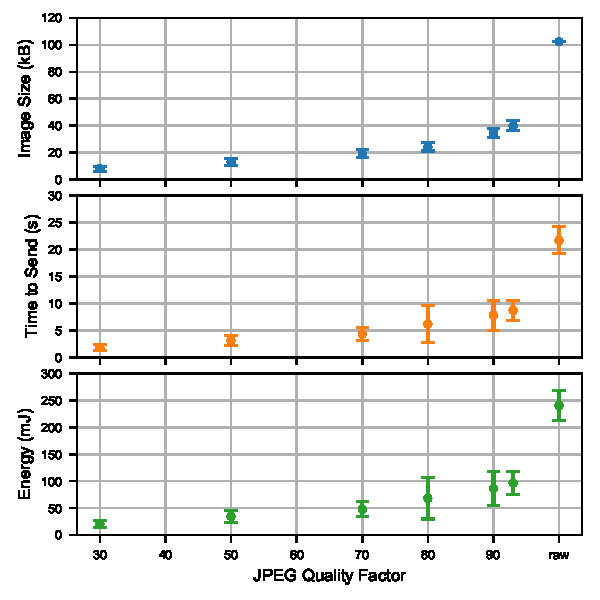
\includegraphics[width=\columnwidth]{figs/permacam/figs/size_time_energy.pdf}
    \caption{Effects of JPEG compression on image size, time to send, and energy to send.
        \normalfont{
            Compression provides exponential decrease in image size, which directly relates to decreases in the time and energy required to send images. Using a low quality factor results in images that are 8.2\% the size of the original raw image. The amount of time and energy required to send images exhibit more variance than image size. This is the result of occasional packet loss and backoff during image transmission. Larger images require more packets and thus a higher probability of this occurring.
        }}
\end{definefigure}

\begin{definefigure}{fig:ssim}
    \centering
    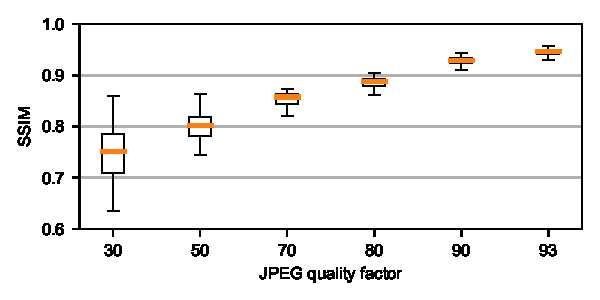
\includegraphics[width=\columnwidth]{figs/permacam/figs/jpeg_ssim.pdf}
    \caption{\normalfont{The image structural similarity index (SSIM) of images compressed at various JPEG quality factors.
        A higher SSIM indicates that an image is a closer representation to the original raw image.
        While a low quality factor results in smaller compressed images, it results in a significant loss in image structural similarity. Quality factors 90 and 93 provide a >90 SSIM, suggesting that they are near identical representations of the original image.
    }}
\end{definefigure}

\begin{definefigure*}{fig:lifetime}
\centering
\begin{subfigure}{0.445\textwidth}
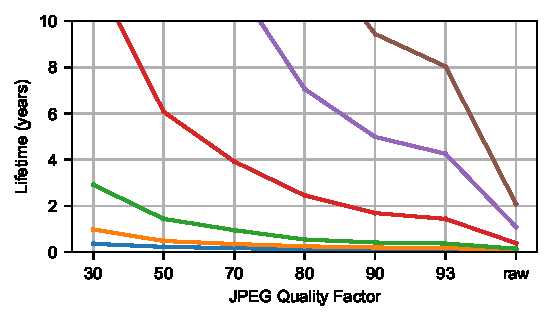
\includegraphics[width=\linewidth]{figs/permacam/figs/lifetime_periodic.pdf}
\label{fig:lifetime_periodic}
\vspace{-1.5\baselineskip}
\caption{Periodic}
\end{subfigure}
%
\begin{subfigure}{0.545\textwidth}
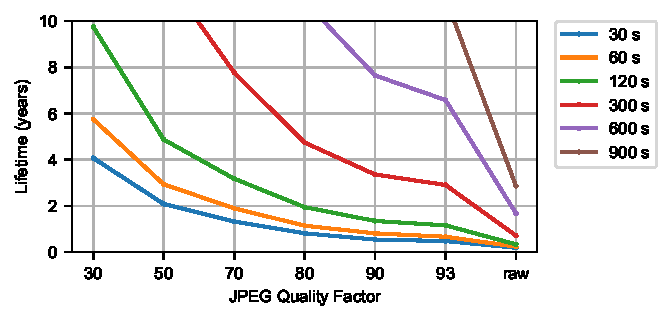
\includegraphics[width=\linewidth]{figs/permacam/figs/lifetime_event_60.pdf}
\label{fig:lifetime_event}
\vspace{-1.5\baselineskip}
\caption{Reactive}
\end{subfigure}
\vspace{-1\baselineskip}
\caption{\normalfont{
    Estimated lifetime from a numerical model. Two workloads are simulated: periodic and reactive. A periodic workload takes a picture at a fixed interval, while the reactive workload models motion events captured by a PIR sensor. We vary the quality factor of images sent, which has a direct impact on the lifetime of the workloads. Each colored line represents a different period of the periodic workload, or the duration of the back off after an event for the reactive workload. As expected, the reactive workload results in a longer lifetime as it captures and transmits fewer images in times of less activity like nighttime. For both workloads, \name is able to transmit images compressed at quality 90 and still achieve a one to five year lifetime based on period or back off duration.
}}
\end{definefigure*}

\begin{definefigure}{fig:multiple}
    \centering
    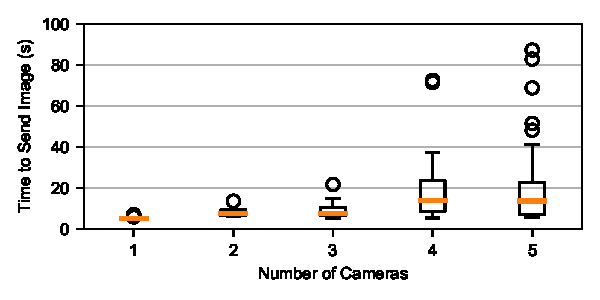
\includegraphics[width=\columnwidth]{figs/permacam/figs/multiple_cameras.pdf}
    \vspace{-2\baselineskip}
    \caption{\normalfont{An image's time to send as number of \namecs on the network increases. All sensors are within one meter radius of each other, and configured to capture and transmit images on motion events to generate the worst case collision condition. Images are compressed with quality 90.
    }}
\end{definefigure}

\begin{definefigure}{fig:map}
    \centering
    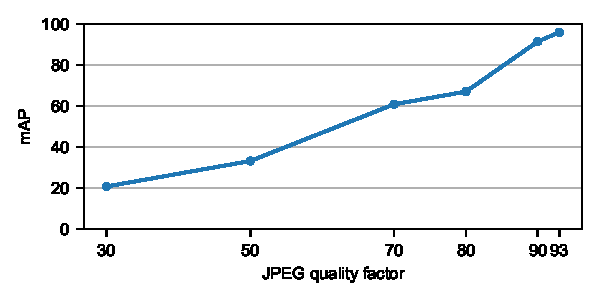
\includegraphics[width=\columnwidth]{figs/permacam/figs/jpeg_mAP.pdf}
    \vspace{-2\baselineskip}
    \caption{\normalfont{Mean Average Precision (mAP) of YOLOv3 person detection on compressed images compared to original raw versions. An IoU of 0.5 is used. Based on the qualitative and quantitative results of image similarity from \cref{fig:compression} and \cref{fig:ssim} it is surprising that mAP degrades so quickly as the compression quality factor decreases. A quality factor of 90 or higher is necessary to achieve the near the same detection performance as a raw image}}
\end{definefigure}

\begin{definefigure}{fig:distance}
    \centering
    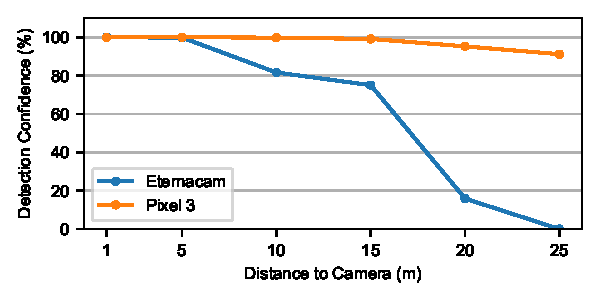
\includegraphics[width=\columnwidth]{figs/permacam/figs/distance_detection.pdf}
    \caption{\normalfont{
        Detection confidence as distance from camera to person is increased. Compared to a modern smartphone camera, the camera on \name can not compete due to limited resolution. However, images captured by \name still enable person detection at a distance of 15-20 meters. This distance is generally sufficient for most indoor spaces.
    }}
\end{definefigure}

\begin{definetable}{tab:local-inference}
\begin{tabularx}{\columnwidth}{l c c c c c}
Dimension (pixels) & Latency (s) & MOPs & Energy (mJ) & Memory (kB) & Accuracy (\%) \\
\hline
48 & 1.72 & 0.450 & 17.2 & 73.7 & 68.6 \\
72 & 2.71 & 1.01 & 27.0 & 91.0 & 69.2 \\
96 & 3.64 & 1.80 & 36.4 & 115. & 72.4 \\
120 & 5.10 & 2.81 & 50.9 & 146. & 74.7 \\
\end{tabularx}
\caption {
    Latency, millions of operations, energy, peak memory, and accuracy 
    of local person classification. Images must be downscaled from full resolution, as inference on a 320x320 image requires too much runtime memory. The quantized version of model weights are used to measure accuracy of the validation set. The highest accuracy achieved is only 74.7\%, and requires 5.1 seconds of continuous computation.
}
\end{definetable}

\begin{definetable}{tab:end-to-end}
\setlength\tymin{1cm}
\small
\begin{tabulary}{\columnwidth}{l c c c}
Compression\newline Quality & Size\newline(kB) & Latency\newline(s) & Energy\newline(mJ) \\
\hline
30  & 1.98 & 0.513 & 4.23\\
50  & 3.25 & 0.764 & 6.95\\
70  & 4.82 & 1.12 & 10.3\\
80  & 6.19 & 1.31 & 13.2\\
90  & 9.12 & 1.86 & 19.5\\
93  & 10.6 & 2.13 & 22.7\\
raw & 25.6 & 4.91 & 54.7\\
\end{tabulary}
\caption {\normalfont{Time and energy required to send 160x160 images end-to-end. Images are compressed with varying JPEG qualities. Sending compressed images requires less time and energy than performing person classification on lower resolution images.}}
\end{definetable}

\begin{definefigure}{fig:cycle-per-byte}
    \centering
    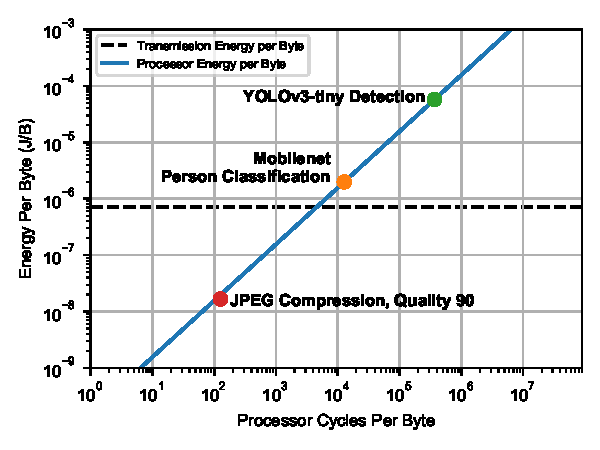
\includegraphics[width=\columnwidth]{figs/permacam/figs/cycles_per_byte.pdf}
    \caption{The required energy per byte of image data to run different algorithms on the processor used by \name{}.
        \normalfont{
            The slope of the solid line represents the energy per cycle of the processor. The dashed line represents the energy per byte of a compressed transmission of an image. Three algorithms are plotted here: JPEG compression with quality factor 90, our custom MobileNets v1 person classifier, YOLOv3-tiny object detection. We estimate the cycles and energy required of YOLOv3, as it requires more memory than available on our microcontroller.
        }}
\end{definefigure} 

We evaluate \name{} on our goals of deployability and capability through a number of experiments. We begin with an analysis of the effects of JPEG compression on image size, time to send, and energy. From this analysis, we use these measured metrics to estimate platform lifetime using different representative workloads. 
%We estimate platform lifetime using different configurations of workloads and image compression. 
We explore the capability of the platform by writing an object detection application on top of the \name{} end-to-end image transfer architecture. We evaluate the ability to detect objects in images captured by \name{} at varying qualities of compression and distance from the camera. We also implement local image inference in the form of person classification. We evaluate the performance of local classification, and compare it to image transmission.
%into the options for reducing energy spent transmitting images, including image compression and downsampling. We analyze the effects of these techniques have on resulting image quality. Based on the efficacy of image compression, we estimate lifetime using a simulation of \name{} to evaluate the longevity of the platform. We evaluate the capability of the platform by performing object detection tasks on the images that it captures. We measure the effects of design decisions on the accuracy of detections.  

\placefigure{fig:size-time-energy}

\subsubsection{Image Compression}
\label{eval:compression}
A raw, full frame image from \name{}'s camera is over 100\,kB in size. Sending these raw images requires a significant amount of time and energy. We employ JPEG compression to significantly reduce image size. This decrease in size comes at the cost of reduced image fidelity and color representation.

We use the Moodstocks JPEC encoder to compress captured images in JPEG format. JPEC is a monochrome JPEG encoder, and we have configured \name{} to use the color version of the HM01B0 image sensor. The images captured are a "mosaiced" color filter array, and performing monochrome JPEG compression on a mosaiced image reduces color representation in addition to image fidelity. JPEG can be configured with different quality factors from 1 to 100. A lower quality factor results in a less accurate representation and smaller compressed size. Image size relates linearly to the time and energy required to send images. 
We configure \name to capture images, compress them with 6 different JPEG quality factors and transmit them. We collect 60 images, each with 6 compressed versions, and analyze the effect of compression on image size, time to send, and energy to send.
The results are displayed in \cref{fig:size-time-energy}. 

\placefigure{fig:compression}

JPEG image compression allows an exponential decrease in image size with respect to the quality factor.
Compressing images at a high quality factor (JPEC's default 93) results in greater than a 2x reduction in image size, time to send, and energy required. There are diminishing gains after the knee of the curve at quality 90, but an image compressed with quality 30 is only 8\% the size of a raw image, on average. Image compression on mosaiced images from \name also does not appear to degrade the perceived quality of the image. We display four compressed and raw versions of the same image in \cref{fig:compression}. Qualitatively, and from a distance, these images appear nearly identical. However, closer inspection reveals artifacts and a significant loss in color fidelity with lower compression quality factors. Quality 93 and a raw image are nearly identical, while quality 30 is more obviously a lower quality compression. However, the important details in the image are preserved and still visible to the human eye.

\placefigure{fig:ssim}

To more quantitatively analyze the effects of compression on mosaiced images, we measure the Structural Similarity Index (SSIM)~\cite{wang2004image} of all 360 compressed images compared to their raw counterparts. SSIM is often used to measure the quality degradation of images due to compression or transmission. The results are summarized in \cref{fig:ssim}. A higher SSIM indicates that an image is a closer representation to the original raw image.
Even with a low quality factor of 30 or 50, the SSIM for images average above 0.75. With an image compressed with a high quality factor, the perceived similarity is above 0.9 and, as seen in \cref{fig:compression}, is almost indistinguishable from the raw image. These results suggest that using a quality factor of 90 or above on to compress images on \name is advantageous if we can afford the energy to send them.

\subsubsection{Camera Density}
While our numerical model can provide an accurate estimate of lifetime, it makes an important assumption. In our modelling, we assume that every image transfer requires the same amount of time and energy. The reality is that wireless environments can have interference, especially for low bandwidth networks like 802.15.4. The result of interference from other networks, devices, or other \namecs, means that packets will be dropped and retransmissions are necessary. This extends the length of image transmission and the increases required energy. 
We explore the scalability and effects of interference when multiple \namecs on the same network. We place all cameras within a meter radius of each other facing the same direction. The network consists of only one Thread router. Each \name is configured to simultaneously capture on a motion event to generate a worst-case collision scenario. Each camera is sending images compressed with quality factor 90.
%In real deployments, cameras are likely to be sparser and multiple Thread routers will be deployed for greater coverage. 
The \namecs are configured with a 2 minute backoff period after a motion event and camera capture. At the start of the experiment, a person walks into view of all the cameras, triggering them simultaneously. The person then remains in view of the cameras for half an hour. We vary the number of cameras active and measure the average time to send images over the duration of the experiment. The results are displayed in \cref{fig:multiple}.

\placefigure{fig:multiple}

We do not currently implement any application layer collision avoidance and we use the default 802.11.4 CSMA MAC protocol specified by Thread. Based on our naive implementation, having more than three \name sensors connected to a single router and on the same network leads to a dramatic increase in time to send images. Implementing an actual coordination protocol between \namecs would dramatically reduce collisions. Additionally, the use of  TCP instead of CoAP block would significantly reduce transmission latency and possible overlap.
%Luckily, during a CoAP backoff period after a missed packet, \name can return to a low power sleep mode, waiting for the back off to expire. 
Irregardless of these improvements, we expect most deployments of \name will be aware of the limitations and will only require one to two cameras per room.

%\subsubsection{Image downscaling}
%\hl{I only downscaled to 160x160 for comparison with local inference, is it worth it to mention here? Could just plot on same figures as above section}

\subsubsection{Object Detection Performance}
To illustrate the capability of the platform and end-to-end image transfer system, we evaluate the ability to perform object detection with \name. The images produced by \name are published over an MQTT stream, which feeds into a script that performs object detection using the pre-trained YOLOv3 network included in the Python ImageAI package \cite{ImageAI}. We do not wish to measure the accuracy and performance of the ImageAI YOLOv3 model, but instead isolate the ability to perform detections on images captured by \name's camera and the effects of different compression quality factors on detection performance.

\placefigure[t]{fig:map}

\subsubsection{Compressed detection accuracy}
While we measure the structural similarity of compressed images using SSIM, this does not directly relate to the performance of object detection on compressed images. To evaluate the effect of image compression on detection accuracy, we use the same 360 images used previously to measure the effects of JPEG compression. These images feature various representative objects of the classes supported by the YOLOv3 model in ImageAI. To quantify the effects of compression, we calculate the mean average precision (mAP) using an intersection overlap union (IOU) of 50\% of the detections compared to a raw image from \name. 
The metrics mAP and IoU=0.5 are both common metrics used to evaluate object detection algorithms. We refer readers unfamiliar with this metric to the Pascal VOC challenge paper~\cite{everingham2010pascal}.

%For a given detection, a bounding box is created. The IoU of this bounding box compared to ground truth is the ratio of the area of overlap to the area of the union between both bounding boxes. Currently, it is common to consider an IoU above 0.5 to be a true positive detection. Average precision (AP) is calculated by integrating the precision/recall curve of the detection results for a class. The mean AP (mAP) is the mean of all calculated AP
In \cref{fig:map}, we display the mAP for different JPEG quality factors. Surprisingly, images compressed with a lower quality factor perform much worse than their SSIM suggests. Images compressed with quality factor 30 and 50 achieve less than 40\% mAP, while factors above 90 achieve near identical detections to their raw counterparts.

\subsubsection{Limitations of resolution}
\name{}'s camera is limited in resolution and color representation compared to most image sensors in modern cameras and cell phones. For example, the Google Pixel 3 features a 12.2 megapixel image sensor, which offers two orders of magnitude more resolution than the HM01B0's 0.1 megapixel. A lower resolution places a limit on the size of objects and the distance at which they can be detected. If an object is only represented by a few pixels, there is unlikely to be enough information to successfully detect it. To evaluate the capability to perform object detection with images captured by \name{}, we compare detection accuracy to images captured by a modern cell phone camera. We successively capture images of a person at varying distances and measure the resultant detection accuracy, if any. The results are summarized in \cref{fig:distance}.

A person is successfully detected at a distance of 20 meters with images from \name{}, though confidence is only 16\%. Unsurprisingly, a person is easily detected at all distances tested with images taken by a Pixel 3. While images captured by \name{} can not compete with the resolution of those captured by cell phones, they are sufficient for detection at reasonable distances. Many indoor spaces do not have sight lines longer than 20 meters, and if they do, additional camera coverage can help mitigate the lack of resolution of a single camera. The ability to clearly depict objects in the distance is partially dependent on the lens configuration of a camera. During this experiment, \name{} was configured with a 200\textdegree\xspace wide angle lens. Better performance could be achieved with a lens with a narrower field of view and more magnification, at the cost of less coverage. We envision most applications will prioritize field of view to cover large areas instead of additional magnification.

\placefigure[t]{fig:distance}

\subsubsection{Local Inference}
\label{eval:localinf}
In addition to end-to-end image transmission, \name is also capable of local image inference. We implement and train a modified MobileNets v1 network using TensorFlow in Python~\cite{tensorflow2015-whitepaper} and the Visual Wake Word dataset~\cite{chowdhery2019visual}. Using TensorFlow Lite for Microcontrollers, we quantize and deploy the model to \name's processor.

We upload 20 images from the validation set to \name, and measure inference latency and energy. We measure inference accuracy across our validation set of 8059 images, using quantized weights in TensorFlow.
%perform inference on images and measure the latency, energy, and accuracy of predictions.  
The results are summarized in \cref{tab:local-inference}. Inference on the largest image dimension (120) requires just over 5 seconds of continuous computation and has a peak memory usage of 146\.kB to achieve a 75.1\% accuracy. This accuracy pales in comparison to what can be achieved with a full sized model running on more powerful hardware. Can local inference provide benefits to energy or latency to make up for its lackluster accuracy?

To answer this question, we also perform end-to-end image transmissions on \name to compare. Images are downsampled from 320x320 to 160x160 to compare with the downsampled images used for inference. They are 1.77x as large as the 120x120 images used for classification. Images are compressed using JPEG at varying qualities. We measure time and energy required to send images. The results of this experiment are summarized in \cref{tab:end-to-end}. Surprisingly, the average energy required to transmit images of this size is generally less than performing inference on them. 
%Generally, performing local person classification on images requires more time and energy than transmitting a compressed version of the image.
For example, we are able to transmit a 160x160 image compressed at quality 93 for under half the energy needed to perform inference on a smaller 120x120 image.
Considering the effort to deploy machine learning inference to a microcontroller, the marginal accuracy of shrunken models, and the demanding energy requirements, a simpler and more beneficial solution is to just transmit images to more capable endpoints.

\placefigure{tab:local-inference}

\subsection{To send or not to send}
This conclusion is unique to the design choices made for \name{} and its envisioned indoor application space. For example, outdoor applications have access to significantly more harvestable energy, but also have different, often higher power, options for wireless communication. Therefore, we seek to provide a generalizable guiding methodology for determining if a device should perform local computation or just send data in entirety based on the kind of applications that designers want to enable. This determination depends on several data points, including processor and radio power, data size, and desired algorithms to run on sensed data.
Most of these parameters are fixed based on component selection and power requirements. Component selection of processor, radio and camera define the \uA/MHz of the processor (52\,\uA/MHz), radio TX current (4.7\,mA), and data size (320x320, 102.4\,kB raw or \textasciitilde35\,kB compressed at quality 90) for \name. We are interested in applying several algorithms on collected image data, including image compression, classification, and detection. We present a metric, cycles per byte, that represent how many processor cycles per byte of data are required for different algorithms. This metric must be measured from microbenchmarks of the algorithm on the desired processor, or estimated from required (FL)OPs of the algorithm and the ISA of the processor.

In \cref{fig:cycle-per-byte}, we plot the energy required for algorithms based on their cycle per byte metric. We plot horizontal lines that represent the amount of energy required to compress and send images. We also display a linear trendline that represents the increasing energy cost per byte of data as more cycles of \name's processor are required. This trendline gives us the inflection point where transmitting data requires the same amount of energy as performing an algorithm of a given cycles per byte of image data. We also plot points for specific algorithms, including image compression, classification, and detection. Note that this figure is plotted on a log-log scale due to the disparity of algorithm complexity.
From this figure, it is clear that our desired inference algorithms require more energy than simply transmitting an image. Beyond just energy, transmitting these images allows us to use full sized and high accuracy versions of models. Additionally, deploying these models to microcontrollers requires significantly more effort than using high level APIs exposed by popular machine learning frameworks like TensorFlow and Pytorch~\cite{8675201}.

\placefigure{tab:end-to-end}

\subsection{Summary}
\hl{TODO: make this more of a summary of the entire permacam section...}
Through many experiments, we evaluate \name's deployability and capability. For deployability, we demonstrate the effectiveness of image compression on image size and resulting time and energy to transmit images. We find that with high compression quality factors, images sent by \name are nearly indistinguishable from raw images, and are half the size. We use these results to inform a numerical model which we use to estimate lifetime of the the \name platform under periodic and reactive workloads. Our model produces an estimated lifetime of 5 to 10 years with compression using quality factor 90, and a period of 10-15 minutes, or a back off of 5-10 minute. We also evaluate the effect of compression on the resulting usefulness of images for object detection. We find that high quality compressed images produce near identical detection results to raw images, and also find that \name is able to produce images that allow a person to be detected at 20 meters, despite the low resolution of its image sensor.

In addition to end-to-end image transmission, we also evaluate \name on its capability of performing local image classification. We find that it is possible to deploy a neural network for person detection on \name. However, the resulting accuracy is only 74.7\% and the required energy to perform this inference is more than double what is required to simply transmit an image. We conclude our evaluation with a generalizable framework and metric, "cycles-per-byte". This framework helps ground decisions about when to process data locally, or send elsewhere for remote processing.

%Recent improvements in microcontrollers go beyond lower power improvements\cite{kim2018system}. Many embedded processors now include hardware floating point, single cycle multiplies, and data-parallel instruction (SIMD) support. The promise of new dedicated accelerators provides the potential of significant improvements in inference performance on low power systems~\cite{armm55,himaxwiseeye}. This has led to renewed interest in performing complex local inference on a battery budget, especially as transmitting large data like images is traditionally very expensive. However, radios have also become far more power efficient, which again muddies the conventional wisdom. Indeed, it is now much cheaper to transmit large data to a more capable system. Desktop or server class machines handily outclass their low power microcontroller and accelerator brethren on performance, providing the ability to perform more complex and accurate inference, if only data can be efficiently delivered to them.
%%Regardless of recent improvements, microcontroller and accelerator performance will continue to pale in comparison to desktop and server class computing systems. 
%This is especially true as memory has not scaled at the same pace as processing.
%This rapidly changing design space points to a requirement for a flexible architecture and framework for thinking about what applications are most suited for local processing versus cloud offload.
%% or data transmission.
%
%In this section, we present \name, the first wireless, energy-harvesting camera platform capable of capturing and transmitting an image every ten minutes for half a decade in indoor environments.
%\name represents a culmination of recent work on low power camera sensors~\cite{josephson2019wireless,nardello2019camaroptera,naderiparizi2015wispcam} and energy harvesting sensor platforms~\cite{jackson2019capacity}. \name features a hierarchical energy harvesting system that couples a small rechargeable battery with a backup non-rechargeable battery. This combination provides the system with a long and reliable lifetime. The longevity and reliability of the platform make it suitable for long-term, low-maintenance deployments. Images captured by \name are capable of driving applications like people detection and counting. 
%With default, pretrained weights, an object detection model is able to detect a person in \name images from 20 meters away.
%
%\name is capable of performing both local inference and transmitting full images end-to-end to more powerful systems. Local inference potentially requires less energy than image transmission, and also provides significantly better privacy guarantees. In cases where privacy is not as much of a concern, image transmission to a more capable endpoint increases the flexibility and performance of inference run on images. Privacy can still be guaranteed if images are transmitted only within a local network.
%We examine the implications of both architectural choices with respect to capability, energy, and latency.
%
%Our results show that on modern SoCs, transmitting images surprisingly enables longer lifetimes and improved inference. While this conclusion is unique to indoor wireless camera sensors 
%whose footprints are not dominated by their energy harvester or storage, its general methodology can be applied to other application spaces as well.
%%
%Through this conclusion, we develop an end-to-end architecture that makes images captured by \name accessible to data collectors and application builders. \name provides a scalable and easily deployable method to quickly gather visual data for machine learning training or datasets. Images collected by \name are easily integrated into popular computer vision and machine learning frameworks like OpenCV, TensorFlow, and PyTorch. Using these tools, high level applications can be built to drive visual applications like building occupancy counting for more efficient energy management and critical infrastructure monitoring atop a long-lived deployment of wireless \name devices.

\section{Summary}

\hl{TODO}